\documentclass[fontsize=12pt,		% Font size
			   toc=listof,			% List of... into table of contents % listofnumbered
			   paper=A4,			% A4 paper
			   headinclude=true,	% Include header into type area calculation
			   footinclude=false,	% Don't include footer into type area calculation
			   headsepline=true,	% Separating line between header and text
			   footsepline=false,	% Separating line between footer and text
			   DIV=calc,			% Auomatically calculate DIV
			   %BCOR=15mm,			% Binding correction
			   %twosided=true,
			   %open=right
			  ]{scrartcl}

\usepackage[english,ngerman]{babel}
\usepackage[utf8]{inputenc}
\usepackage[T1]{fontenc}

\usepackage{lmodern}
\usepackage{microtype}

\usepackage{textcomp}				% Avoids conflicts between siunitx and microtype
\usepackage{siunitx}				% Allow for german decimals, e.g. 1,344 instead of 1.344 + other stuff

\usepackage{graphicx}
\usepackage{listings}
\usepackage{color}
\usepackage{hyperref}

% Autorenangabe
\newcommand\mychapter[2]{\chapter{#2}\vspace{-1.5em}\hspace{2.1em}\emph{#1}\vspace{1.5em}}
\newcommand\mysection[2]{\section{#2}\vspace{-0.9em}\hspace{2.1em}\emph{#1}\vspace{1.5em}}
\newcommand\mysubsection[2]{\subsection{#2}\vspace{-0.5em}\hspace{3.2em}\emph{#1}\vspace{1.3em}}

% ToDO

\newcommand\todo[1]{\footnote{\textcolor{red}{\textbf{#1}}}}

% PDF Metadaten

\pdfinfo{
 /Title (BlinkenTiles)
 /Author (Fabian Gärtner, Sarah Häfele, Alexander Scheurer, Linda Schey, Johannes Winter, Meike Zöckler)
}

\begin{document}

%%%%%%%%%%%%%%%%%%%%%%%%%%%%%%%%%%%%%%%%%
% University Assignment Title Page 
% LaTeX Template
% Version 1.0 (27/12/12)
%
% This template has been downloaded from:
% http://www.LaTeXTemplates.com
%
% Original author:
% WikiBooks (http://en.wikibooks.org/wiki/LaTeX/Title_Creation)
%
% License:
% CC BY-NC-SA 3.0 (http://creativecommons.org/licenses/by-nc-sa/3.0/)
% 
% Instructions for using this template:
% This title page is capable of being compiled as is. This is not useful for 
% including it in another document. To do this, you have two options: 
%
% 1) Copy/paste everything between \begin{document} and \end{document} 
% starting at \begin{titlepage} and paste this into another LaTeX file where you 
% want your title page.
% OR
% 2) Remove everything outside the \begin{titlepage} and \end{titlepage} and 
% move this file to the same directory as the LaTeX file you wish to add it to. 
% Then add \input{./title_page_1.tex} to your LaTeX file where you want your
% title page.
%
%%%%%%%%%%%%%%%%%%%%%%%%%%%%%%%%%%%%%%%%%

%----------------------------------------------------------------------------------------
%	PACKAGES AND OTHER DOCUMENT CONFIGURATIONS
%----------------------------------------------------------------------------------------

%\documentclass[12pt]{article}

%\begin{document}

\begin{titlepage}

\newcommand{\HRule}{\rule{\linewidth}{0.5mm}} % Defines a new command for the horizontal lines, change thickness here

\center % Center everything on the page
 
%----------------------------------------------------------------------------------------
%	HEADING SECTIONS
%----------------------------------------------------------------------------------------

\Large Hochschule Furtwangen - Fakultät Digitale Medien\\[0.5cm] % Name of your university/college
{\Large \bfseries Interaktionsdesign}\\[0.5cm] % Major heading such as course name
\large Wintersemester 2014/15\\[0.5cm] % Minor heading such as course title

%----------------------------------------------------------------------------------------
%	TITLE SECTION
%----------------------------------------------------------------------------------------

\HRule \\[0.2cm]
%{ \huge \bfseries BlinkenTiles}\\[0cm] % Title of your document

\includegraphics[width=0.5\textwidth]{images/logo_final}\\[-0.35cm]
\HRule \\[0.7cm]
 
%----------------------------------------------------------------------------------------
%	AUTHOR SECTION
%----------------------------------------------------------------------------------------

\begin{minipage}{0.55\textwidth}
\begin{flushleft} \large
%\emph{Authoren:}\\
Fabian Gärtner, MIM1\\
Sarah Häfele, MIM1\\
Alexander Scheurer, MIM1\\
Linda Schey, MIM2\\
Johannes Winter, DIM1\\
Maike Zöckler, DIM1\\

\end{flushleft}
\end{minipage}
~
\begin{minipage}{0.4\textwidth}
\begin{flushright} \large
%\emph{Supervisor:} \\
Prof. Patricia Stolz\\
Prof. Dr. Matthias Wölfel\\ % Supervisor's Name
\end{flushright}
\end{minipage}\\[2cm]

% If you don't want a supervisor, uncomment the two lines below and remove the section above
%\Large \emph{Author:}\\
%John \textsc{Smith}\\[3cm] % Your name

%----------------------------------------------------------------------------------------
%	DATE SECTION
%----------------------------------------------------------------------------------------

{\large \today}\\[3cm] % Date, change the \today to a set date if you want to be precise

%----------------------------------------------------------------------------------------
%	LOGO SECTION
%----------------------------------------------------------------------------------------

%\includegraphics{Logo}\\[1cm] % Include a department/university logo - this will require the graphicx package
 
%----------------------------------------------------------------------------------------

\vfill % Fill the rest of the page with whitespace

\end{titlepage}
%\end{document}

\section*{Abstract}
Die vorliegende Arbeit stellt die Dokumentation zur Konzeption und prototypischen Umsetzung von \emph{BlinkenTiles} dar. BlinkenTiles ist eine großflächige Installation, die es Personen erlaubt, durch eine auf den Boden projizierte Sound-Matrix und durch das Tracking einer Microsoft Kinect mit dem eigenen Körper Musik zu machen. Die Installation wurde im Rahmen der Veranstaltung \textit{Interaktionsdesign} in den Masterstudiengängen \textit{Design Interaktiver Medien} sowie \textit{Medieninformatik} an der Fakultät Digitale Medien der Hochschule Furtwangen im Wintersemester 2014/2015 unter der Betreuung von Frau Prof. Stolz und Herrn Prof. Dr. Wölfel entwickelt.

\tableofcontents

%Bitte im folgenden \includes{} nutzen!

\clearpage
\section{Grundidee}
\subsection{Ideenfindung}
\subsection{Zielsetzung}
\subsection{Werbebotschaft}
\subsection{Strategische Planung}

\clearpage
\section{Planung und Skizzierung}
\subsection{Zielgruppenanalyse}
\subsection{Tests}
\subsection{Technischer Aufbau}

\clearpage
\section{Umsetzung des Prototypen}
\mysubsection{Das Team}{Softwaretechnische Entscheidungen}
\label{ssec:entscheidungen}

Zur Entwicklung der Anwendung für den Prototypen fiel die Entscheidung auf die 3D-Game-Engine Unity\footnote{\url{http://www.unity3d.com}}. Gründe hierfür waren u.\,a., dass der Umgang mit Unity den meisten Projektmitgliedern aus anderen Lehrveranstaltungen geläufig war und die Anbindung externer Softwarebibliotheken (z.B. das \emph{Microsoft Kinect}-SDK oder \emph{OpenCV} zur Personenerkennung, vgl. Seite \pageref{sec:objdet}) über \CS{} als Programmiersprache vergleichsweise einfach ist. Zudem wurde entschieden Git als Sourcecode-Verwaltung einzusetzen, wodurch der Programmcode von BlinkenTiles jederzeit online abrufbar ist\footnote{\url{https://github.com/InformatischesQuartett/BlinkenTiles}}. Die wichtigsten Einstellungen in BlinkenTiles können über eine externe Konfigurationsdatei vorgenommen werden. Dadurch können alle Parameter, die in den folgenden Abschnitten näher erläutert werden (vgl. Abschnitte~\ref{ssec:DMX}, \ref{sec:tiles} und \ref{sec:objdet}), geändert werden, ohne dass die komplette Anwendung noch einmal kompiliert und exportiert werden muss.

Für die Kommunikation mit den LED-Scheinwerfern wurde \emph{Freestyler}\footnote{\url{http://www.freestylerdmx.be/}}, eine kostenfreie und umfangreiche DMX-Lichtsteuerungs-Software verwendet, da diese für das verwendete DMX512-Interface in der Produktbeschreibung empfohlen wurde und einwandfrei kompatibel ist. Außerdem bietet Freestyler die Möglichkeit per Befehl problemlos aus anderen Programmen (hier die BlinkenTiles-Anwendung) heraus auf Funktionen zuzugreifen, diese zu steuern und so die LED-Scheinwerfer anzusprechen. Mehr dazu im folgenden Abschnitt.


\mysubsection{Sarah Häfele}{Aufbau}

Die Installation besteht aus mehreren Hardware- und Software-Komponenten und soll hier mit Hilfe einer kurzen, modellhaften Übersicht, die den endgültigen Aufbau des Prototypen zeigt, skizziert werden. Die darauf folgenden Kapitel gehen anschließend näher auf die einzelnen Komponenten ein. Der Prototyp der Installation wurde am 20.01.2015 im Rahmen des \textit{Tag der Medien} der Fakultät Digitale Medien aufgebaut und getestet. Auf zwei Ebenen wurden Gerätschaften installiert, damit die Besucher schon beim Eintreten mit akustischen und visuellen Reizen konfrontiert und zum Mitmachen bewegt wurden. Die zwei Grafiken zeigen das Erdgeschoss und den ersten Stock des Gebäudes.
\begin{figure}[htbp]
	\centering
		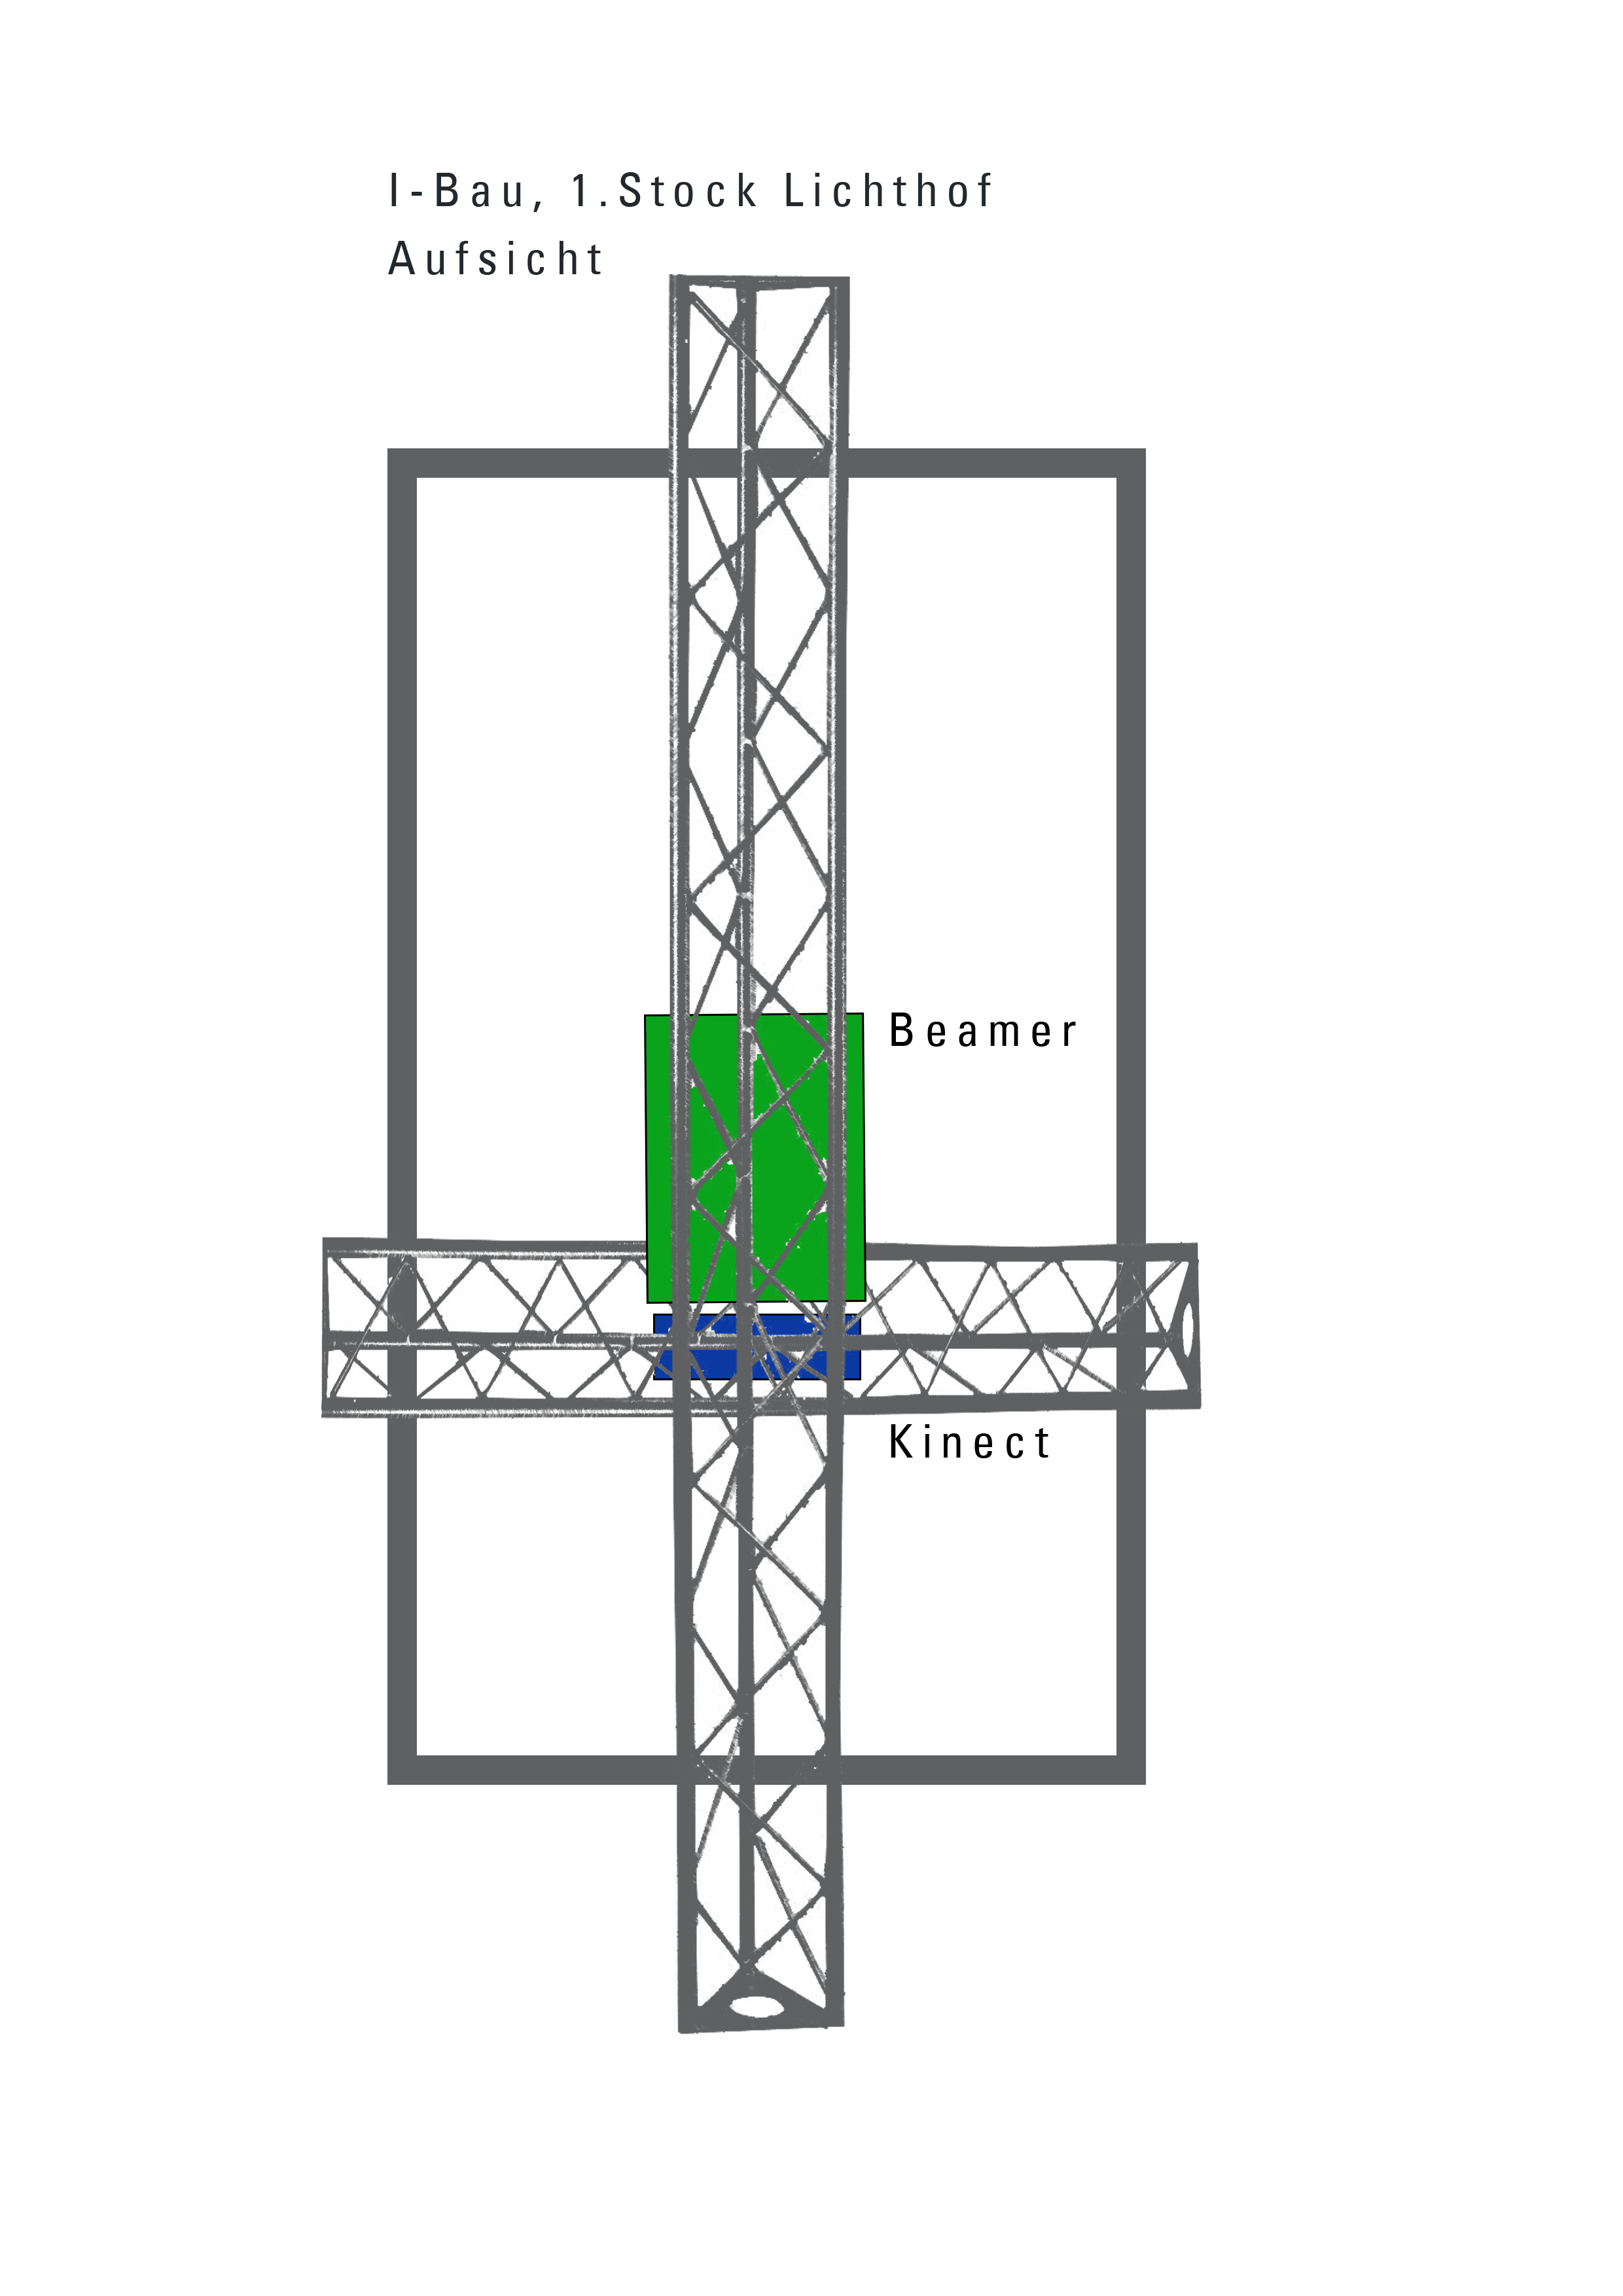
\includegraphics[width=0.88\textwidth]{images/ModelFirstFloor.png}
	\caption{Aufbau der Installation im 1.Stock des I-Baus}
	\label{fig:ModelFF}
\end{figure}

Im ersten Stockwerk hängt über dem Lichthof eine zwei Meter lange Traverse, getragen von zwei Stativen, in deren Mitte ein Epson EB-4950WU Beamer (in der Abbildung \autoref{fig:ModelFF} grün markiert) an einer speziell von der Werkstatt der Hochschule angefertigten Metallhalterung in das Erdgeschoss des Gebäudes strahlt. Der Beamer, eine Leihgabe des Kreismedienzentrums Villingen, kann mit seiner Farbhelligkeit von bis zu 4.500 Lumen und eine Auflösung von 1920 x 1200 Pixeln den dunklen Boden des I-Baus mühelos ausleuchten und ist zudem für längere Betriebszeiten ausgerichtet. Durch die erhöhte Stellung der Traversenstative hängt der Beamer sechs Meter über dem Erdgeschossboden.\\
Auf der Brüstung des Lichthofes liegt im 90° Winkel dazu eine ein Meter lange Traverse. Sie wird nicht ganz mittig zu der längeren Traverse ausgerichtet, damit die mit Spannfix daran befestigte Microsoft Kinect v2 (in der Abbildung in blau markiert) nicht das Bild des Beamers stört und wird durch Holzhalterungen und Doughty-Clamps fixiert. Durch die direkte Anbringung auf dem Geländer des Lichthofes, hängt die Kinect zudem auf 4,5 Meter Höhe und kann so bequem die Bewegungen der im Erdgeschoss befindlichen Personen aufnehmen.\\
Zudem sind zwei Scheinwerfer (so genannte \textit{Revos}, in Abbildung \autoref{fig:ModelFF} braun markiert ) an der längeren Traverse links und rechts vom Beamer angebracht und versehen den Boden mit zusätzlichen Lichteffekten, indem sie auf den Musiktakt reagieren.\\
Die Geräte sind per HDMI-Kabel an einen PC angeschlossen, auf welchem das in der Spieleengine Unity geschriebene Kontrollprogramm läuft (hierzu in den folgenden Kapiteln mehr).

\begin{figure}[htbp]
	\centering
		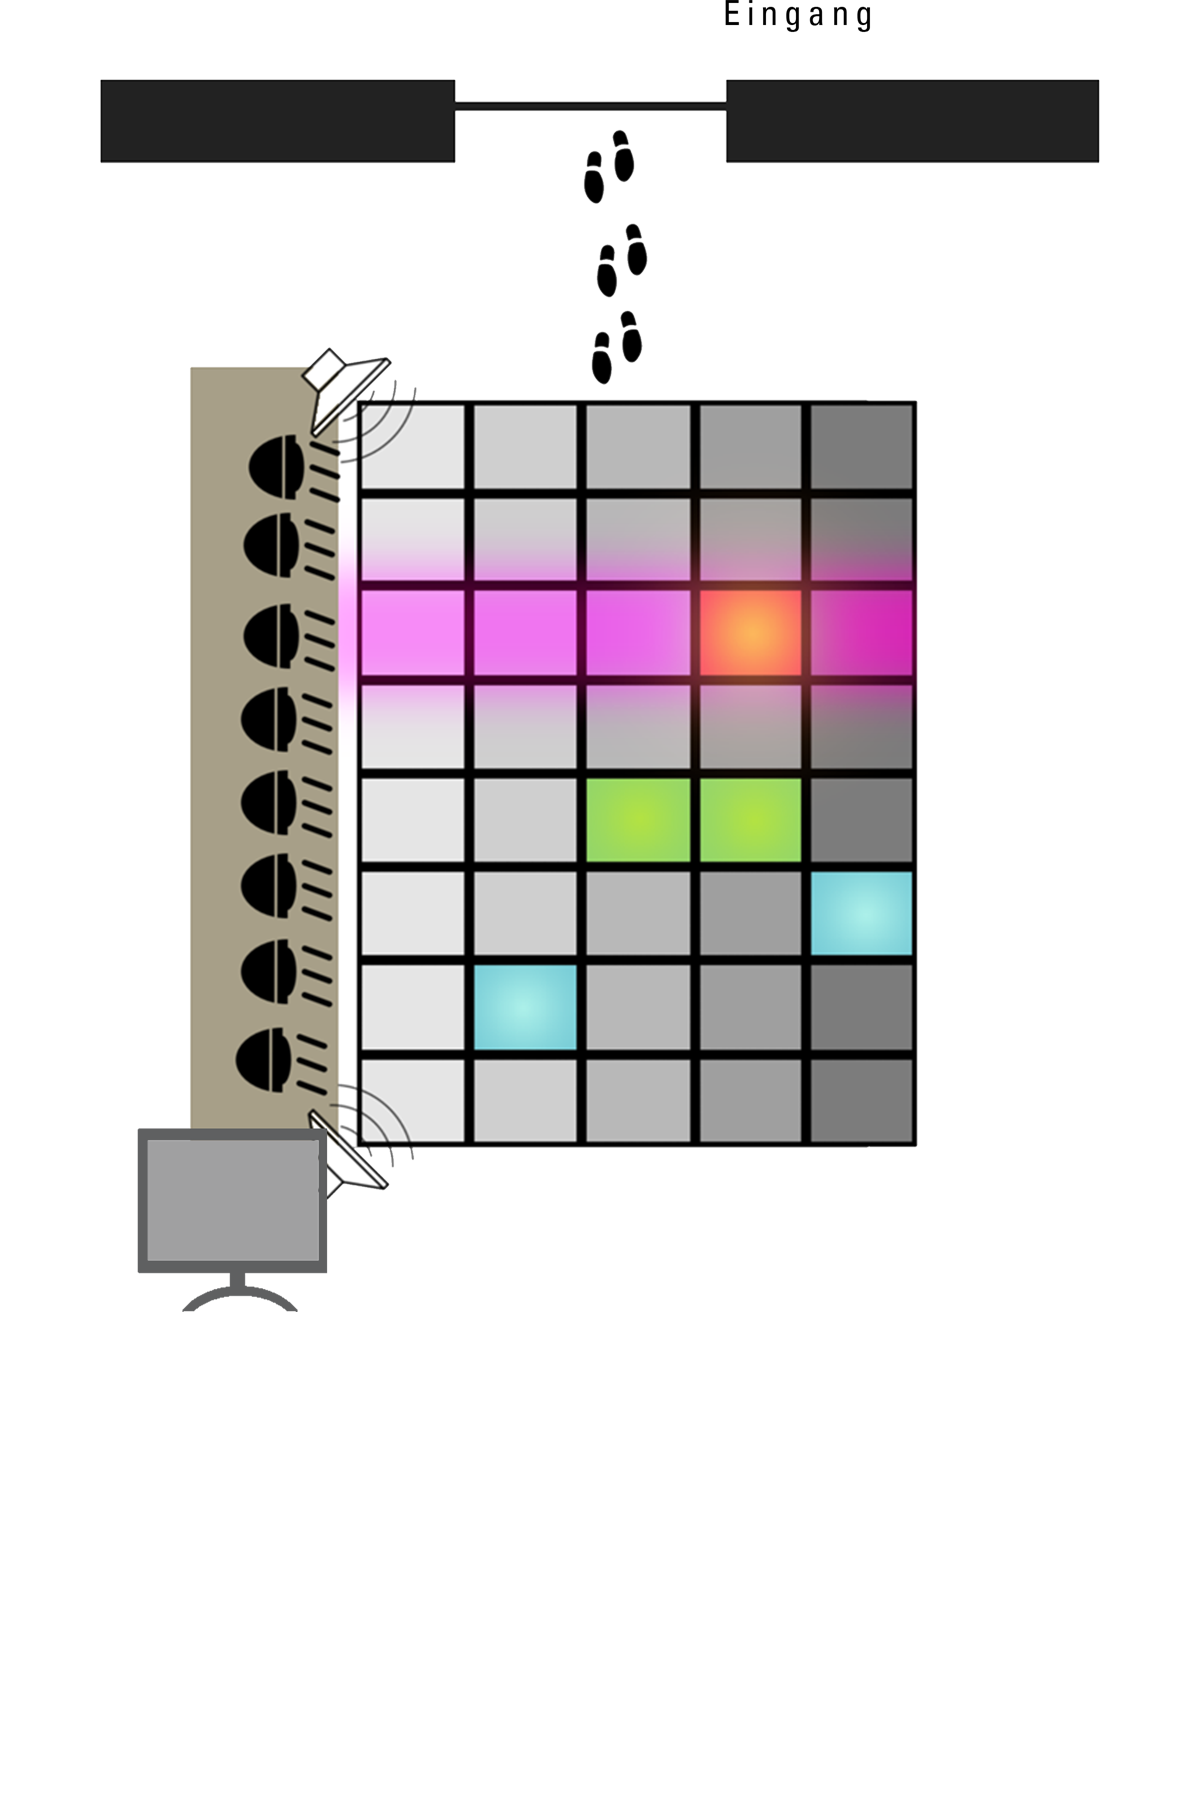
\includegraphics[width=1.0\textwidth]{images/ModelGroundFloor.png}
	\caption{Aufbau der Installation im Erdgeschoss des I-Baus}
	\label{fig:ModelGF}
\end{figure}

Im Erdgeschoss (siehe Abbildung \autoref{fig:ModelGF}) wird durch den Beamer ein 5 x 8 flächiges Raster projiziert, welches die einzelnen Töne repräsentiert. Acht LED-Scheinwerfer untermalen die Rhythmuslinie, welche bestimmt, wann ein Ton abgespielt wird. Die Scheinwerfer sind durch ein DMX-Interface untereinander und mit dem Computer verbunden und werden durch ein eigenes Programm gesteuert (siehe \autoref{ssec:ssec:DMX}).\\
Ein großer LED-Monitor zeigt den Besuchern Informationen an und dient zusätzlich als Motivation (siehe auch \autoref{ssec:CtA}).\\
Die Musik wird durch einen mobilen, jedoch leistungsstarken Radiorekorder (auch: \textit{Boombox} genannt) abgespielt.
\mysubsection{Linda Schey}{Ansteuerung Scheinwerfer}
\label{ssec:DMX}

Für die LED-Scheinwerfer wurden acht \emph{Eurolite LED CLS-18 QCL RGBW} verwendet, die jeweils über einen dreipoligen XLR- Ein- bzw. Ausgang verfügen, so dass sie in Reihe geschaltet über das DMX512 Protokoll mit zwölf Kanälen gesteuert werden können. Ein \emph{Eurolite USB-DMX512-PRO} Interface dient als Schnittstelle zwischen den Lichtern und dem PC. Angesteuert werden die Lichter dann mittels der in \autoref{ssec:entscheidungen} bereits erwähnten Software Freestyler. \autoref{fig:FStoLED} zeigt grob wie die drei Komponenten zusammenhängen. Es wird hier den Pfeilen der Abbildung entsprechend nur in eine Richtung kommuniziert, da das Verhalten der Scheinwerfer ausschließlich durch die Applikation gesteuert wird und keine rückläufige Kommunikation nötig ist.
\begin{figure}[htbp]
	\centering
		
\includegraphics[width=0.90\textwidth]{images/FStoDMXInterfaceToLEDs.PNG}
	\caption{Verknüpfung der Komponenten}
	\label{fig:FStoLED}
\end{figure}
Jeder Scheinwerfer besteht aus 18 LEDs die in drei Reihen mit jeweils sechs LEDs angeordnet sind. Zwei Zeilen, also sechs LEDs, werden in der Applikation jeweils als ein Segment verwendet und kann mit vier Farbkanälen separat angesteuert werden. Insgesamt werden 12 Farbkanäle pro Scheinwerfer eingesetzt. Innerhalb der \enquote{Blinken Tiles} Anwendung gibt es zwei Klassen, die hauptverantwortlich für die Lichtsteuerung sind. \emph{Spot.cs} und \emph{LightController.cs}. \emph{Spot.cs} repräsentiert in der Anwendung einen LED-Scheinwerfer. Diese Klasse verwaltet die Farbwerte für jeden einzelnen Spot und dessen Segmente. In der Klasse \emph{LightController.cs} werden die Farbwerte für alle acht Scheinwerfer in einem Array gespeichert. Dieses Array wird mit den Farbwerten der einzelnen Scheinwerfer befüllt. Die Farbwerte der Scheinwerfer, werden regelmäßig pro Frame aktualisiert. Dabei wird überprüft welcher der Scheinwerfer gerade aktiv sein muss und anhand einer Zeitreferenz welches Segment des Scheinwerfers aktiviert sein soll. Alle anderen Scheinwerfer und deren Segmente werden aus Schwarz gestellt, also nicht leuchtend. 
Jeder Scheinwerfer besteht aus 18 LEDs die in drei Reihen mit jeweils sechs LEDs angeordnet sind. Zwei Zeilen, also sechs LEDs, werden in der Applikation jeweils als ein Segment verwendet und  kann mit vier Farbkanälen separat angesteuert werden. Insgesamt werden also 12 Farbkanäle pro Scheinwerfer eingesetzt. Innerhalb der \enquote{Blinken Tiles} Anwendung gibt es zwei Klassen, die hauptverantwortlich für die Lichtsteuerung sind. \emph{Spot.cs} und \emph{LightController.cs}. \emph{Spot.cs} repräsentiert in der Anwendung einen LED-Scheinwerfer. Die Klasse \emph{Spot.cs} verwaltet die Farbwerte für jeden einzelnen Spot und dessen Segmente. Welchen Farbwerte eingetragen werden wird aus einer Konfigurationsdatei ausgelesen.. In der Klasse \emph{LightController.cs} werden die Farbwerte für alle acht Scheinwerfer in einem Array gespeichert. Die Farbwerte der Scheinwerfer, werden regelmäßig pro Frame aktualisiert. Dabei wird überprüft welcher der Scheinwerfer gerade aktiv sein muss und anhand einer Zeitreferenz welches Segment des Scheinwerfers aktiviert sein soll (\emph{UpdateFaderValues()}. Alle anderen Scheinwerfer und deren Segmente werden auf Schwarz gestellt, nicht leuchtend. 
Um die Scheinwerfer aus der Anwendung \enquote{Blinken Tiles} heraus zu steuern wird ein Zwischenschritt über die Software Freesyler gemacht, da diese Software die Ansteuerung der einzelnen Segmente eines jeden Scheinwerfers sehr komfortabel gestaltet. Um aus \enquote{BlinkenTiles} mit Freestyler zu kommunizieren wurde eine DLL (\emph{LetThereBeLight.dll}) erstellt, die per \emph{FindWindow()} und \emph{SendMessage()} mit zwischen \enquote{Blinken Tiles} und Freestyler vermittelt.



\mysubsection{Linda Schey}{Multimonitor Support}

Zu Beginn des Projektes wurde versuch eine möglichst große Projektionsfläche zu erhalten. In Ermangelung eines Beamers, der die gewünschte Größe projizieren konnte wurde auf drei Beamer zurückgegriffen, die dann nebeneinander ein jeder ein Drittel der Applikation darstellen sollte. Um dies zu realisieren musste aber das komplette Bild das projiziert werden sollte in drei einzelne Bilder geteilt werden. Da die Beamer nicht nebeneinander, sondern über einander aufgebaut werden sollten, damit das komplette Bild hoch und breit genug ist müssen die erhaltenen Bilder jeweils um 90° gedreht werden. Dafür wurde in Unity eine extra Kamera in die Szene eingefügt, die die Szene als RenderTexture aufnimmt. Diese RenderTexture wurde dann in drei einzelne Texturen getrennt. Jede Textur um 90° gedreht und dann nebeneinander als Gui-Elemente dargestellt. Soweit war diese Funktionalität auch schon implementiert, bis auf kleine Justierungen beim Zuschneiden der einzelnen Teil Texturen. \\
Ein anderer Ansatz war drei um 90° gedrehte Kameras in die Szene zu integreren die jeweils ein Drittel des Spielfeldes filmten. 
\begin{figure}[htbp]
	\centering
		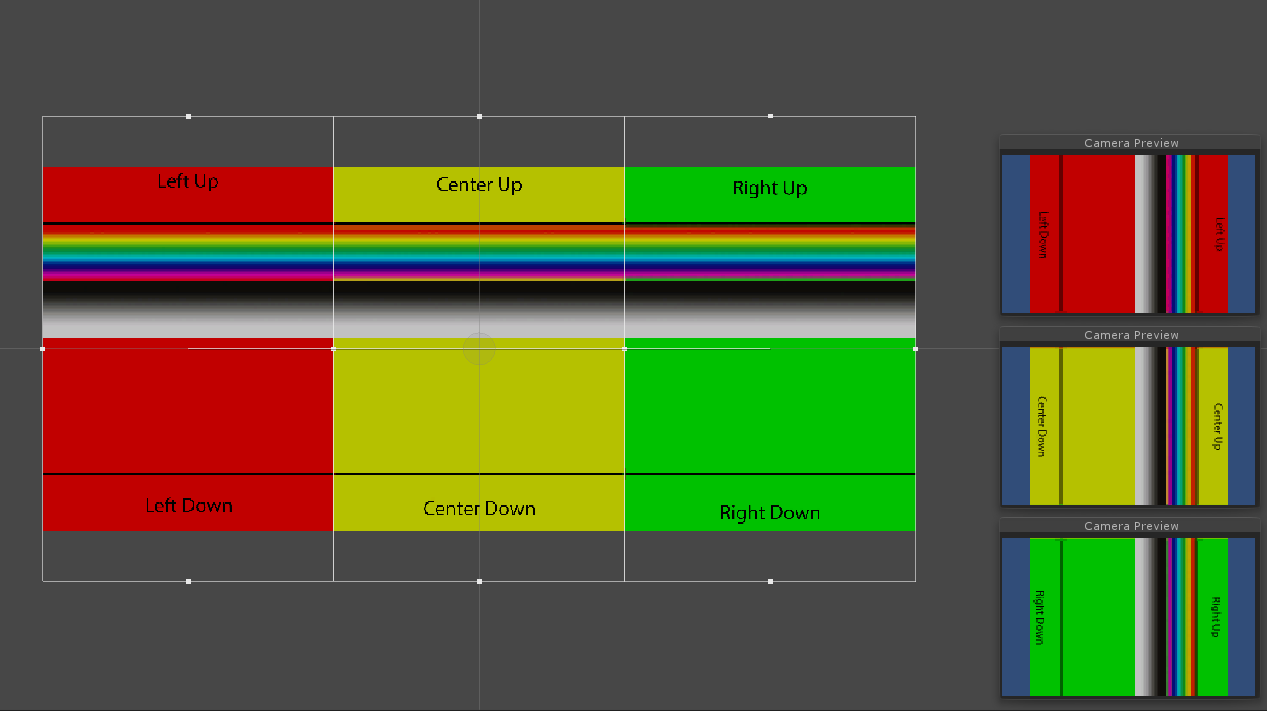
\includegraphics[width=0.8\textwidth]{images/RenderTextureBeispielSzene.PNG}
	\caption{Aufbau der Szene in Unity mit den drein RenderTextrure Ausschnitten am Beispiel eines Dummy Objektes}
	\label{fig:RenderTextureBeispielSzene}
\end{figure}
Daraus erhielt man drei RenderTextures, die dann nebeneinander als Gui rendern werden konnten. Dafür wurde zunächst mit einem Beispiel Objekt gearbeitet, das ein Material zugewiesen bekam, welches es bei der Entwicklung vereinfachte zu erkenne, ob die Kameras richtig ausgerichtet waren und dann auch entsprechend richtig auf die Gui gerendert wurden. 
\begin{figure}[htbp]
	\centering
		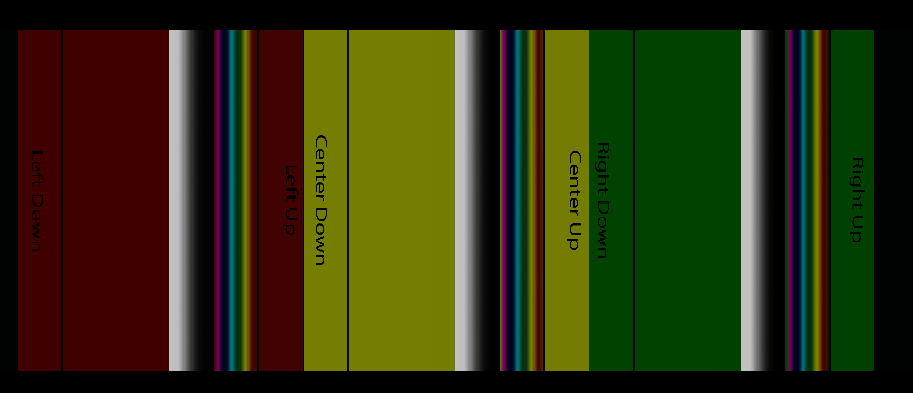
\includegraphics[width=0.8\textwidth]{images/RenderTexturesAlsGui.PNG}
	\caption{RenderTextures nebeneinander auf die Gui gerendert}
	\label{fig:RenderTexturesAlsGui}
\end{figure}\\
Die drei Kameras, mussten jedoch von Hand auf die Szene eingestellt werden, so dass es auch hier wieder zu Ungenauigkeiten hätte kommen können. Andererseits wäre man hier flexibler beim Ausrichten der Szene auf die drei Beamer gewesen, in dem man zum Beispiel die Übergänge zwischen den drei Texturen jeweils so hätte Platzieren können, dass sie auf einem Spalt der Felder des Spielfeldes gelegen wären. Auch dieser Ansatz wurde umgesetzt und hat mit funktioniert allerdings auch mit kleinen Ungenauigkeiten.\\
Beide Ansätze waren jedoch nicht zu 100 Prozent exakt,was das Aufteilten der Szene in drei Teil Texturen betraf. Außerdem standen keine drei identischen Beamer zur Verfügung, sodass es unter den einzelnen Beamern Unterschiede bei der Lichtintensität gab.
Da anstatt der Lösung mit den drei Beamern doch noch ein geeignetes Gerät gefunden wurde, das alleine die gewünschte Projektionsfläche erbrachte, wurde die Idee mit den drei Beamern, sowie die bisherige Implementierung dafür verworfen und ist im finalen Stand des Projektes nicht mehr enthalten.\\
\subsection{Grafische Oberfläche}

Teil der Grafischen Oberfläche ist das Spielfeld (\autoref{fig:gui-tiles}), mit dem die Nutzer wie im Konzept beschrieben, interagieren.

\begin{figure}[htbp] 
  \centering
     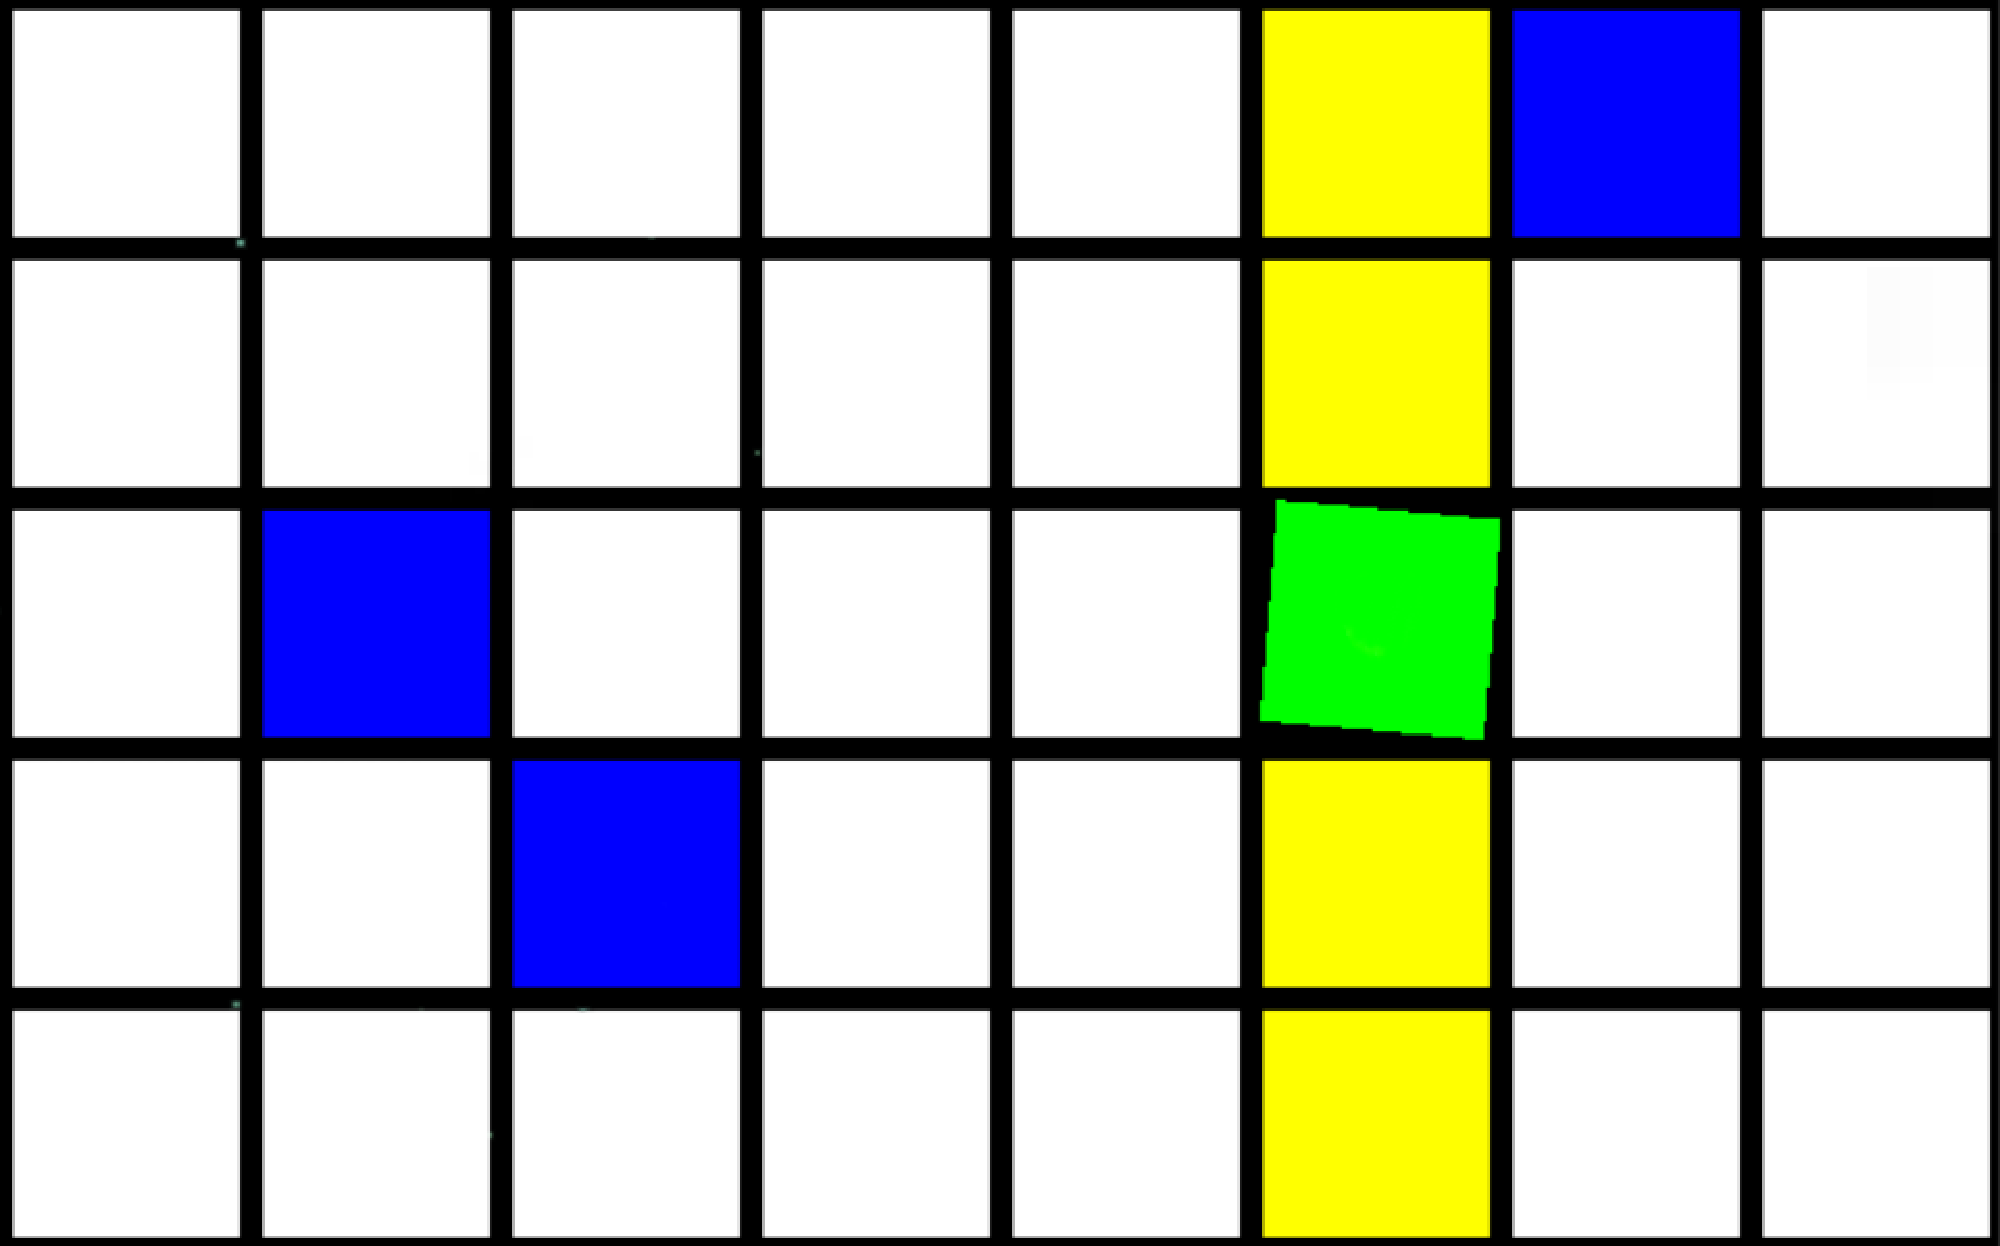
\includegraphics[width=0.9\textwidth]{images/gui-tiles}
  \caption{Das Spielfeld}
  \label{fig:gui-tiles}
\end{figure}
\mysubsection{Alexander Scheurer}{Spielfeld und Felder}
\label{sec:tiles}

Das Spielfeld und die Felder werden von zwei Klassen bestimmt, die TileController und TileBehaviour Klasse. 
Die TileController Klasse ist die Zentrale Klasse, sie beinhaltet die Spiellogik, baut das Spielfeld auf, verarbeitet Eingaben (von Personenerkennung, Maus, Tastatur, Konfiguration und Idle-Mode).

Die Spiellogik umfasst überwiegend das Timing der Abläufe und in Abhängigkeit davon das zuweisen von Zustände an die einzelnen Felder. Die Zustände die Zugewiesen werden beschreiben zum Beispiel ob auf diesem eine Person steht, ob derzeit sich der Zeitindex in der Reihe dieses Feldes befindet oder ob sogar beides vorher genante zutrifft, was zur Folge hätte dass auch der entsprechende Ton zu dem Feld abgespielt werden muss. Die TileController Klasse weist den Feldern den entsprechenden Zustand sequenziell zu:
\begin{enumerate}
\item Alle Felder werden zurückgesetzt (Clear pass)
\item Der Zustand für Zeitimpuls wird bei den entsprechenden Feldern gesetzt (Timer pass)
\item Der Zustand für Feldern auf denen Personen erkannt wurden, werden gesetzt (People pass)
\item Der vereinigte Zustand von 2. und 3. wird gesetzt (Shake'n'Play pass)
\end{enumerate}
Verarbeitet wird dieser Zustand von jedem Feld selbst mit Hilfe der TileBehaviour Klasse. In dieser passiert die Umsetzung von Zustand zu Aktion, also welcher Shader (Farbe) für das Feld gesetzt wird oder soll es wackeln weil es den entsprechenden Zustand vom Shake'n'Play pass zugewiesen bekommen hat.

Zum Start des Spiels hat der TileController die Aufgabe das Spielfeld aufzubauen, dies macht er anhand von JSON-Konfigurationsdateien einmal für die Grundkonfiguration als auch Konfigurationen für jeden Song. Die Grundkonfiguration definiert unter anderem welche Ausmaße das Spielfeld hat, oder auch welche Farbe einem bestimmten Feldzustand zugewiesen ist. Die Song-Konfiguration beinhaltet zum Beispiel die Angabe über die Beats pro Minute und die Pfade zu den Audiodateien.

Benutzereingaben nimmt der TileController entgegen und veranlasst die entsprechende Aktion. Zum Beispiel einen Songwechsel oder das verarbeiten eines Feldzustandes von der Personenerkennung oder dem Idle-Node.



\mysubsection{Sarah Häfele}{Call to Action}\label{ssec:CtA}

Die Vermutung, dass bei einer Installation mit Musik und der Notwendigkeit, sich zu bewegen, die Hemmschwelle diese zu nutzen höher liegt, liegt nahe. Neben Lichteffekten durch die Scheinwerfer und dem offiziellen Spielfeld dienen deswegen weitere Komponenten zur \textit{Call to Action}, also zur Motivation der Besucher. Diese sollen nicht nur zum Mitmachen bewegen, sondern auch gleichzeitig anleitend wirken.

\subsubsection{Der Presentation-Screen}

Der Presentation-Screen ist als eine Art Präsentationsfläche gedacht, die den Nutzern weitere Informationen zur Installation liefern soll. In der Spieleengine Unity mit C\# entwickelt, kann sie als eigenständige Anwendung auf einem großen Bildschirm neben dem Spielfeld angezeigt werden. Die Anwendung besteht bislang aus vier Modi, angefangen mit dem Startmenü, welches das Logo der Installation und weitere Menüpunkte anzeigt. Der \textit{How-To}-Modus zeigt ein Video welches kurz erklärt, wie das Spielprinzip funktioniert, erstellt von Fabian Gärtner in Adobe Premiere mit Grafiken von Sandra Beuck. Im \textit{Behind-the-Scenes}-Modus wird ein aktuelles Bild der Kinect sowie das Beamerbild gezeigt um zu erklären, wie die Technik dahinter funktioniert. Die Anwendung kommuniziert dabei über das Internet mit der BlinkenTiles-Anwendung. Zuletzt zeigt der \textit{Time-Lapse}-Modus ein Video des Aufbaus der Installation, aufgenommen mit einer GoPro Kamera und geschnitten von Fabian Gärtner.\\
Die Modi können in einem Loop abgespielt werden, wobei nach einiger Zeit oder wenn das Video zu Ende ist das Programm in den nächsten Modus springt. Wenn die Hauptanwendung von BlinkenTiles jedoch in den Challenge-Modus wechselt, verändert sich auch der Presentation-Screen: er springt zum \textit{How-To}-Video und zeigt zudem Information zum abgespielten Lied an. Dies beinhaltet den Musiktitel und einen Countdown (siehe Abbildung \autoref{fig:PresScreen}).

\begin{figure}[htbp]
	\centering
		
\includegraphics[width=0.88\textwidth]{images/PresScreen.png}
	\caption{Presentation-Screen im Challenge Mode}
	\label{fig:PresScreen}
\end{figure}

Die BlinkenTiles-Anwendung kommuniziert mit einem XML-File über das Internet mit dem Presentation-Programm. Die Hauptanwendung erstellt das File und legt es in einem Netzwerkordner ab. Dieser Teil wurde von Linda Schey implementiert. Die Presentation-Anwendung greift auf das File zu, parst die Textinformationen und speichert sie in entsprechenden Variablen. Abbildung \autoref{fig:PresScreen} zeigt ein minimales Beispiel, welche Informationen so an den Presentation-Screen übermittelt werden können.

\begin{figure}[htbp]
	\centering
		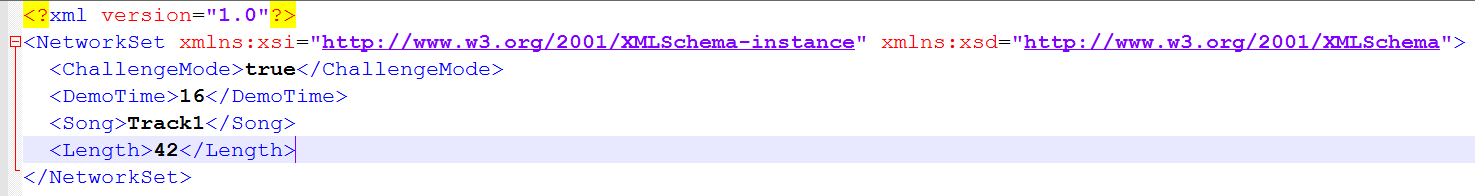
\includegraphics[width=1.0\textwidth]{images/XML.png}
	\caption{XML-File mit aktuellen Informationen für den Presentation-Screen }
	\label{fig:PresScreen}
\end{figure}

Die Variablen werden dann an die einzelnen Codeelemente weitergegeben und für die Anzeigen verwendet. Der Countdown wird durch die übermittelte Länge des Liedes ermittelt und dann selbstständig dekrementiert. Endet der Challenge Mode, wird der Loop normal fortgesetzt.

\subsubsection{Spielfeld}
Das Spielfeld, welches durch den Beamer auf den Boden projiziert 
idle animation
Code

als presentation
\mysubsection{Fabian Gärtner}{Personenerkennung mittels Microsoft Kinect}

Zur Erkennung von Personen auf dem Spielfeld mittels Microsoft Kinect konnten keine Standardfunktionen verwendet werden, da das Kinect-SDK den Einsatz der Kinect aus der Vogelperspektive nicht vorsieht. Stattdessen muss das von der Kinect aufgenommene Tiefenbild mittels Bildverarbeitungstechniken auf Personen bzw. verallgemeinert gesprochen auf Objektkonturen hin untersucht werden. In BlinkenTiles sind dafür die drei Klassen \enquote{KinectManager}, \enquote{BlobDetection} und \enquote{BlobDetectionThread} zuständig. Erstere fragt unter Anwendung des Kinect-SDKs von Microsoft das Tiefenbild (30 Bilder pro Sekunde mit einer Auflösung von 512 x 424 Pixel) und -- bei Bedarf -- das Farbbild (15 Bilder pro Sekunde mit einer Auflösung von 1920 x 1080 Pixel) der Kinect ab. Das Tiefenbild ist dabei ein zweidimensionales Array, das mit Werten zwischen 0 und 8000 die pro Pixel gemessene Tiefe in Millimeter angibt. Da sich die Farbkamera von der Tiefenkamera in Auflösung und Bildwinkel unterscheidet, müssen die Werte des Farbbildes, um beide Bilder übereinander legen zu können, mittels einer vom Kinect-SDK bereitgestellten Funktion umgerechnet werden. Auch diese Funktionalität und die Möglichkeit, Tiefenbilder in Form von Dateien abzuspeichern und für den Fall, dass die Kinect nicht angeschlossen ist, als Testdaten zu verwenden, stellt die Klasse bereit.

Die Weiterverarbeitung des Tiefenbildes und damit die eigentliche Bildverarbeitung findet in der Klasse \enquote{BlobDetectionThread} statt und wird zur Laufzeit in einem eigenen Thread ausgeführt. Dies war zu Beginn der Entwicklung noch notwendig, da die anfangs prozessorlastige Objekterkennung zu einer niedrigen Bildrate in der Hauptanwendung führte und damit auch Auswirkungen auf den Spielablauf und das Abspielen der Musik hatte. Dieser Prozess konnte im Verlauf der Entwicklung aber stetig optimiert werden, sodass die Bildverarbeitung auf eine Dauer von lediglich 12 Millisekunden pro Tiefenbild reduziert werden konnte. Mit etwas mehr als 80 Bildern pro Sekunde liegt die Objekterkennung damit bereits weit über der Bildrate der Kinect mit rund 30 Bildern pro Sekunde und kann ohne Verzögerung und in Echtzeit stattfinden. Die Auslagerung in einen eigenen Thread wurde aber beibehalten, sodass die Arbeitslast auch weiterhin gleichmäßig auf mehrere CPU-Kerne verteilt wird und mögliche Verzögerungen bei der Abfrage der Tiefenbilder keine Auswirkungen auf die Hauptanwendung und den Spielablauf haben.

Hauptsächlich für die Bildverarbeitung verwendet wird die kostenfreie Open-Source-Bibliothek OpenCV, die über den C-Sharp-Wrapper EmguCV angesteuert wird. OpenCV erlaubt die Anwendung von Algorithmen und grundlegenden mathematischen Operationen auf Matrizen und Bilder. Konkret wird bei BlinkenTiles zunächst das als Array vorliegende Bild gefiltert und normalisiert. Die Filterung arbeitet anhand vom Nutzer eingestellter Werte für minimale und maximale Tiefe. Alle Werte über und alle Werte unter diesen Vorgaben werden auf 0 gesetzt, sodass diese die Erkennung nicht weiter stören. In der Praxis kann damit ein stark reflektierender Boden herausgefiltert werden. Die anschließende Normalisierung hilft, den Kontrast des Tiefenbildes zu erhöhen und so die dann folgende Binarisierung des Bildes zu optimieren. Auf das binarisierte Bild wird letztlich die Konturerkennung von OpenCV angewendet, die Objekte ab einer bestimmten Größe erkennt und ein entsprechendes Konturrechteck zurückliefert. Dieses Rechteck kann anschließend mit den Feldern der Matrix abgeglichen werden und bei Überschneidungen zwischen Konturrechteck und einem Feld das Feld aktiviert werden. Jeder dieser Schritte ist vom Nutzer über eine im Folgenden näher erläuterte GUI separat darstellbar und konfigurierbar, um eine optimale Objekterkennung zu ermöglichen. Des Weiteren werden regelmäßig die einzelnen Schritte als Bilder herausgespeichert, sodass sie den Spielern über den Präsentationsbildschirm angezeigt werden können.

Die Klasse \enquote{BlobDetection} schließlich ist hauptsächlich für die Verwaltung der grafischen Benutzeroberfläche (GUI) der Bildverarbeitung und die Verwaltung der eben beschriebenen Klassen zuständig. Dieser Teil der GUI, wie er in Abbildung X auf Seite X dargestellt ist, nimmt die linke Hälfte der gesamten GUI von BlinkenTiles ein und erstreckt sich damit über einen Monitor. Die GUI stellt das Tiefenbild in seiner ursprünglichen Form oder nach einem der zuvor beschriebenen Verarbeitungsschritte, bspw. in binarisierter Form oder mit farbigen Konturrechtecken um erkannte Objekte, dar. Des Weiteren erlaubt die GUI über eine Reihe von Slidern die Einstellung von Filterwerten, Spielfeld- und Feldergröße sowie Spielfeldposition. Ebenso kann ein Raster über dem Tiefenbild dargestellt werden, bei dem alle aktivieren Felder, also alle Felder auf denen Personen erkannt wurden, farbig markiert sind. Um dieses Raster dem vom Beamer erzeugten Spielfeld anzupassen, also um Beamer und Kinect zu synchronisieren, besteht die Möglichkeit eine Überlagerung von Farb- und Tiefenbild anzuzeigen, die dann die Anpassung der Größe und Ausrichtung des Rasters auf dem Tiefenbild mittels der Slider erlaubt. Alle Einstellungen können auch zuvor über die externe Konfigurationsdatei geladen werden.

\subsubsection{Aufgetretene Probleme}

Am Tag der Medien zeigte sich, dass die Tische, auf denen u.\,a. die LED-Scheinwerfer standen, aufgrund ihrer hellen Oberfläche nicht aus dem Tiefenbild herausgefiltert werden konnten und daher ebenfalls als Objekte erkannt wurden. Dies führte dazu, dass Personen, die auf einem der Felder in der Nähe der Tische standen, zusammen mit den Tischen als ein großes Objekt erkannt und dadurch gelegentlich zu viele Felder gleichzeitig aktiviert wurden. Beheben ließe sich das Problem, indem das Tiefenbild vor der weiteren Verarbeitung auf den relevanten Bereich, also auf Spielfeldgröße zugeschnitten wird. Auch hierfür könnten entsprechende Regler in die GUI integriert werden, sodass der Zuschnitt manuell und je nach Bedarf eingestellt werden kann.

Ein weiteres Problem ist die Perspektive, vor allem dann, wenn die Kinect nicht mittig über dem Spielfeld hängt. So funktioniert die Erkennung von Personen, die sich direkt unter der Kinect befinden zwar tadellos, je weiter eine Person aber von der Kinect entfernt ist, desto mehr Felder deckt sie aufgrund der schrägen Aufsicht gleichzeitig ab. Eine kurzfristige Lösung am Tag der Medien war es, die Felder in der Anwendung größer als in der Realität einzustellen. Des Weiteren wird bereits nicht das ganze Feld auf Überschneidungen mit Konturen überprüft, sondern lediglich ein kleinerer (ebenfalls einstellbarer) Bereich in der Mitte der Felder. Um das Problem aber besser zu lösen, wäre entweder eine zweite Kinect oder eine perspektivisch korrekte Berechnung und ein unsymmetrisches Raster notwendig. So könnten bspw. die Felder des Rasters in den Randbereichen vergrößert oder die Tiefenfilterung zu den Rändern hin verstärkt werden, sodass in diesen Bereichen nur noch die Beine von Personen für die Überschneidung relevant sind, nicht aber der Kopf, der möglicherweise ein anderes Felder überdeckt. Welche Methode sich hier am besten eignet, müsste durch weitere Tests herausgefunden werden.

Störend war auch, dass die Einstellungen zwar wie beschrieben aus einer Konfigurationsdatei geladen werden können, die Werte aber momentan noch per Hand eingetragen werden müssen. Interessant neben einem Button zum Speichern der Einstellungen könnte für eine solche Installation daher auch eine automatische Kalibrierung sein, um bei einem Neustart die manuelle Neukonfiguration zu vermeiden. Technisch ließe sich das über ein vom Beamer dargestelltes Testmuster lösen, das von der Bildverarbeitung erkannt wird und das Raster entsprechend dimensionieren und positionieren lässt. Auch die optimalen Werte für die Filterung könnten so automatisiert ermittelt werden.


\newpage

\begin{figure}[htbp] 
  \centering
     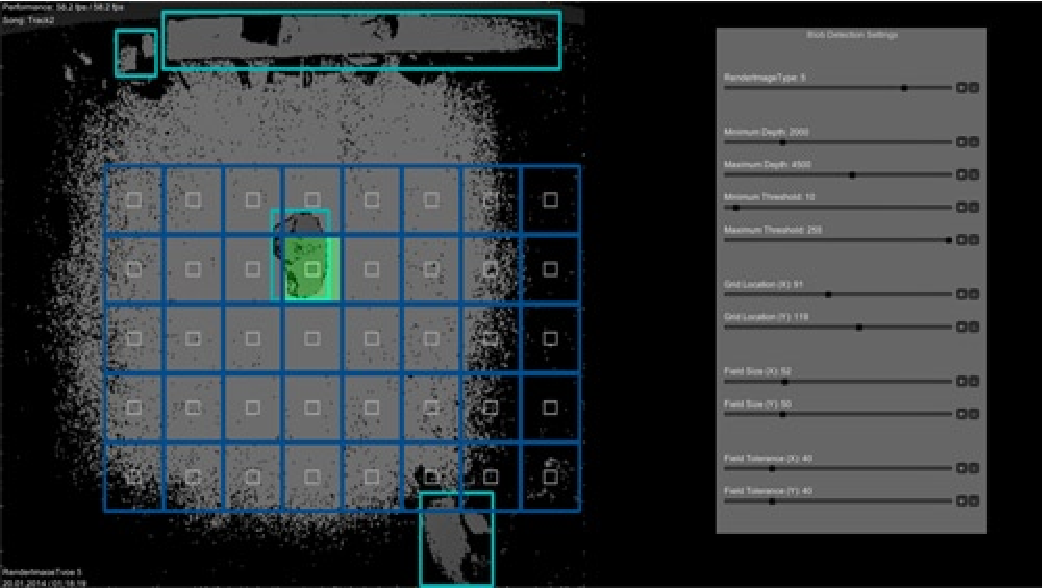
\includegraphics[width=0.9\textwidth]{images/Blob}
  \caption{Schneiden der Spuren in Ableton Live}
  \label{fig:blob}
\end{figure}\todo{caption}

\subsection{Audiogestaltung und Inspiration}
Das Konzept der Installation beruht auf einem klassischen Step-Sequenzer. Solche Sequenzer steuern die Klangerzeugung eines Synthesizers dahingehend, dass sowohl Rhythmus als auch Tonhöhe programmiert werden können. Der Name bezieht sich dabei auf die einzelnen „Steps“ die mit Tönen belegt werden können. Klassische analoge Step-Sequenzer wie der Roland TB 303 bieten 16 Schritte an, womit also pro Durchlauf 16 Töne gespielt werden können. Somit entspricht jeder Schritt einer 16tel Note eines Taktes. Es ist hervorzuheben, dass bei einem Step-Sequenzer die Noteneingabe nicht unmittelbar zu einer Klangerzeugung führt. Stattdessen tastet ein Impuls nacheinander alle „Steps“ ab und übermittelt die Daten an den Klangerzeuger. Nachdem der Impuls einmal durchgelaufen ist, beginnt der er wieder bei dem ersten Step. Dadurch entstehen repetitive Tonfolgen, sogenannte Loops. Step-Sequenzer haben gerade aufgrund dieser Beschränkung zahlreiche Genre wie Acid House, Electronic Body Music und Drum and Bass entscheidend geprägt.

Das Konzept der Installation weicht in mehreren Punkten vom klassischen Step-Sequenzer ab. Zum Einen gibt es statt 16 Schritten nur 8. Außerdem ist die Tonauswahl auf 5 Tonhöhen pro Schritt begrenzt. Des Weiteren wird ist ein Ton nur so lange aktiviert, wie auch eine Person auf dem entsprechenden Feld steht. Das musikalische Konzept berücksichtigt diese Einschränkungen. Da nur 5 Töne gespielt werden können und auch nur 8 Steps zur Verfügung stehen, wird ein Backing Track benötigt, der eine harmonische Grundlage für das Spiel des Instrumentes bietet.

Anspruch der Installation war es aber weniger ein komplexes Instrument zu bieten, viel mehr eine musikalische Spielwiese. Aus diesem Grund liegt die Entscheidung nahe, sich die technischen Beschränkungen zu Nutze zu machen. Es wurde also auf eine Skala zurückgegriffen, die einerseits nur 5 Töne hat und andererseits keine Halbtonschritte aufweist: die Anhemitonische Pentatonik. Der Vorteil liegt darin, dass keine kleinen Sekunden und Tritoni gespielt werden können, die für unsere Hörgewohnheiten „unrein“ klingen. Durch diese Maßnahme wurde also sichergestellt, dass unabhängig von Menge und Position der Benutzer ein recht harmonisches Gesamtbild entsteht, auch wenn dadurch auf die Leittonwirkung einer Diatonik oder Hemitonischen Pentatonik verzichtet werden muss. Außerdem war der Tonumfang natürlich auf eine Oktave beschränkt, mehr als 5 Tonhöhen hätten das musikalische Ergebnis interessanter gestaltet aber auch die Nutzerfreundlichkeit eingeschränkt. Da die Installation in erster Linie intuitiv bedienbar sein sollte, wurde der Tonumfang nicht weiter ausgebaut.

Für den experimentellen Modus der Installation wurden drei Backing Tracks mit jeweils 5 zugehörigen Tonhöhen vorproduziert. Der durchlaufende Impuls wurde auf die Geschwindigkeit des entsprechenden Backing Tracks angepasst und die zugehörigen Töne auf die Felder gemappt. Da der Klangerzeuger kein Synthesizer sondern ein Sampler war, mussten die Einzeltöne im Voraus synthetisiert und gerendert werden. Grundsätzlich wurden eher sphärische Klänge mit langem Nachhall (entweder Reverb oder Hüllkurvengenerator) eingesetzt, da die Benutzer der Installation keinen Einfluss auf die Länge des Tons hatten. In Hüllkurvenparametern gesprochen musste also der Attack deutlich hörbar sein um ein auditives Feedback zu geben, die Sustainlautstärke musste relativ schnell erreicht werden und wesentlich leiser als der Attack sein, damit sich bei mehreren Personen die Sounds nicht zu stark überdeckten. Dadurch wurden relativ perkussive Klänge erzeugt, die durch den Nachhall eine gewisse Stetigkeit erreichten. Die Backing Tracks bildeten das rhythmische und harmonische Grundgerüst und wurden ebenfalls im Voraus produziert und gerendert. Dabei wurde Wert darauf gelegt, zwar eine harmonische Orientierung zu bieten, der Backing Track sollte jedoch keine komplexe harmonische Struktur aufweisen. In den Backing Tracks wurde also ebenfalls weitgehend auf die oben erwähnte Pentatonik zurückgegriffen, um aber ein wenig musikalische Spannung zu kreieren, wurden an ausgewählten Stellen auch Töne aus diatonischen Skalen verwendet.

Für den Challenge Modus wurden ebenfalls drei Backing Tracks und passende Töne vorproduziert, da jedoch die technischen und konzeptionellen Bedingungen andere waren, soll darauf noch näher eingegangen werden. Das Ziel des Challenge Modus ist es, mit der Installation bekannte Lieder nachzuspielen, ähnlich wie bei Guitar Hero. Problematisch ist jedoch, dass die Reaktionsgeschwindigkeit der Benutzer nicht so schnell ist wie es eigentlich nötig wäre. Das größte Hindernis ist jedoch, dass die Nutzer die Installation verlassen müssen, wenn sie keinen Ton spielen wollen. Sobald sie auf irgendeinem Feld stehen und der Impuls dieses erreicht wird der Ton getriggert, auch wenn er falsch ist. Anders gesagt: Die Zustände der Nutzer auf dem Spielfeld sind analog, benötigt wären aber digitale Zustände, an oder aus. Aus diesem Grund mussten Songs gefunden werden, die einerseits recht bekannt sind, ein minimales Tonspektrum aufweisen und langsam genug sind um mit der Installation spielbar zu sein. Die Entscheidung fiel auf „Smoke on the water“ von Deep Purple, „Paint it black“ von den Rolling Stones und “One” von Swedish House Mafia.

Die Ausschnitte der Lieder die benutzt werden sollten, wurden zunächst nachgespielt und aufgenommen. Dabei war es wichtig, hervorstechende Klangeigenschaften der Originale zu berücksichtigen um den Wiedererkennungswert nicht zu verlieren. Bei „Smoke on the water“ wurde beispielsweise ein bekannter britischer Röhrenverstärker mit vorgeschaltetem Overdrive verwendet. Nachdem alle Einzelspuren aufgenommen waren musste bestimmt werden, welche Spuren den Backing Track bildeten und welche Spur von den Nutzern gespielt werden sollte. Der Backing Track wurde dann ohne die entsprechende Spur gerendert. Die Spur die der Nutzer spielen sollte, musste nun in kleine Samples geschnitten werden um auf die verschiedenen Felder aufgeteilt werden zu können.

\begin{figure}[htbp] 
  \centering
     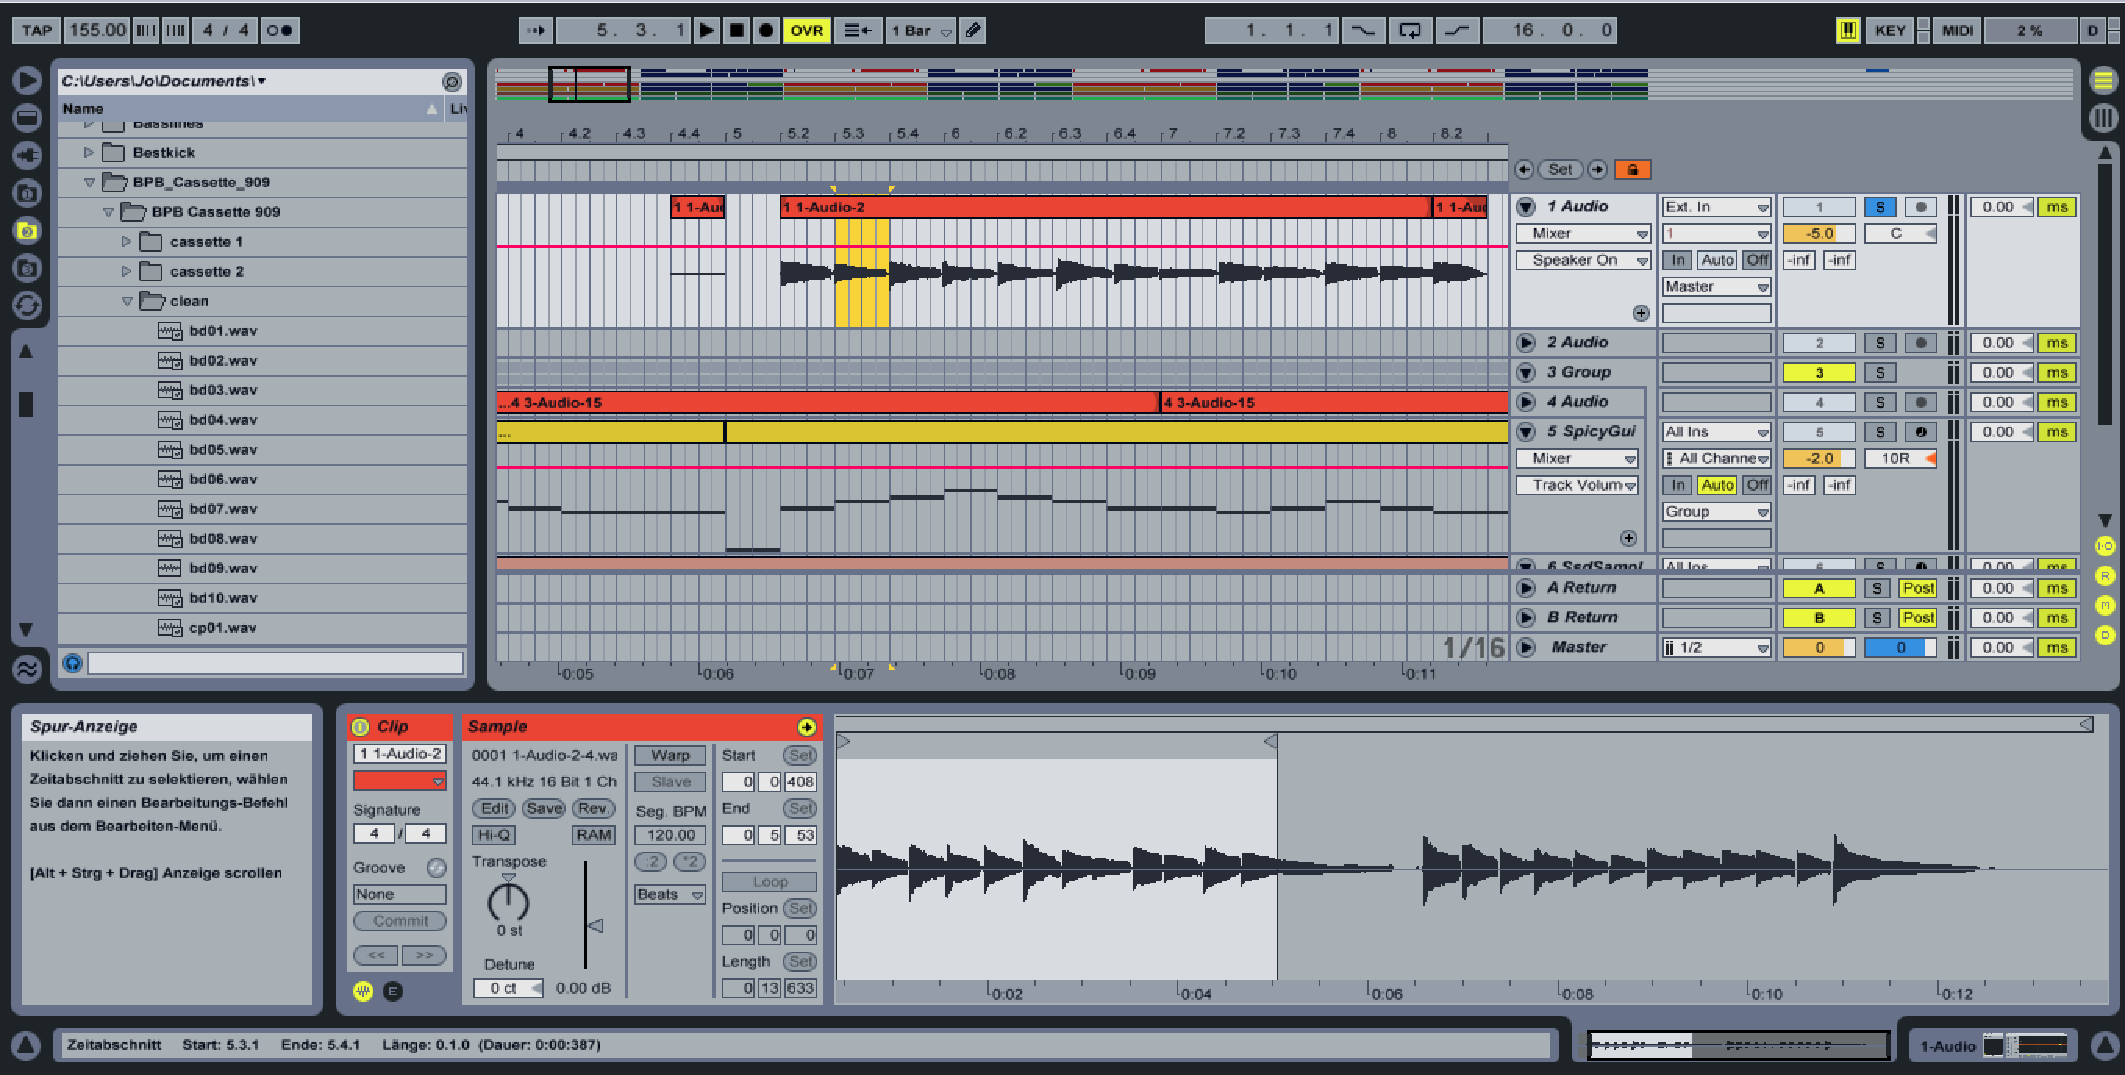
\includegraphics[width=0.9\textwidth]{images/Musikkonzeption}
  \caption{Schneiden der Spuren in Ableton Live}
  \label{fig:audio1}
\end{figure}

Dabei ergaben sich in einigen Fällen Probleme bezüglich der Tonlänge. Da die Schritte des Step-Sequenzers immer auf einen bestimmten Rhythmuswert quantisiert waren, zum Beispiel 8tel oder 16tel Noten, mussten hinsichtlich Synkopen oft Kompromisse eingegangen werden. Bei „One“ führte dies dazu, dass der Impuls so schnell war, dass das Lied damit praktisch unspielbar wurde. Für den Challenge Modus erwies sich damit das Konzept der Soundmatrix insgesamt als relativ ungeeignet, während im experimentellen Modus musikalisch interessante Ergebnisse erreicht wurden.

\clearpage
\section{Tag der Medien}
\subsection{kleiner Bericht mit Fotos}
\subsection{Praxiserfahrungen}

\clearpage
\section{Showreel}
\mysubsection{Das Team}{Aufgaben-Verteilung}

Tabelle \ref{tab:aufgaben} fasst die verschiedenen Aufgabenbereiche bei der Konzeption und Umsetzung von BlinkenTiles zusammen und listet die jeweils Hauptverantwortlichen für die Bearbeitung der entsprechenden Aufgaben. Unterstützt wurden die genannten Personen dabei in der Regel durch die anderen Gruppenmitglieder. Genaueres dazu kann dem Repository auf GitHub oder den einzelnen Kapiteln dieser Dokumentation entnommen werden.

\vspace{0.8em}

\begin{table}[hc]
\begin{center}
\begin{tabular}[hc]{l|l}
\textbf{Aufgabe} & \textbf{Hauptverantwortlich}\\
\hline
Idee und Konzeption& Fabian Gärtner, Sarah Häfele,\\
&Alexander Scheurer, Linda Schey,\\
&Johannes Winter, Meike Zöckler\\\hline
Orga Technik& Fabian Gärtner, Alexander Scheurer\\\hline
Tests und Aufbau& Fabian Gärtner, Sarah Häfele,\\
&Alexander Scheurer, Linda Schey\\\hline
Techn. Zeichnungen& Fabian Gärtner, Sarah Häfele\\\hline
Beamer-Halterung& Mustafa (HFU Werkstatt)\\\hline
Logo und Grafiken& Sandra Beuck\\\hline
Ansteuerung Scheinwerfer&Linda Schey\\\hline
Bau \enquote{Photonenbündler}&Fabian Gärtner, Linda Schey, \\&Meike Zöckler\\\hline
Multimonitor-Support& Linda Schey\\\hline
Personenerkennung& Fabian Gärtner\\\hline
Spielfeld und Tiles& Alexander Scheurer\\\hline
Spiellogik& Alexander Scheurer\\\hline
Idle-Animation& Sarah Häfele\\\hline
Präsentationsbildschirm& Sarah Häfele\\\hline
Netzwerk/XML& Sarah Häfele, Linda Schey\\\hline
Musik& Johannes Winter\\\hline
Kamera \& Schnitt Teaser&Fabian Gärtner, Meike Zöckler,\\&Johannes Winter\\
\hline
\end{tabular}
\caption{Aufgaben Verteilung - Übersicht}
\label{tab:aufgaben}
\end{center}
\end{table}

\clearpage
\section{Fazit}
\mysubsection{Sarah Häfele}{Möglichkeiten zur Weiterentwicklung}

Rhythmische Geschicklichkeitspiele sind heutzutage bei PC- wie auch bei Konsolen-Nutzern beliebt. Als Beispiel sollen hier Spiele wie \textit{Guitar Hero}, \textit{Audiosurf} oder das kürzlich erschienene \textit{Crypt of the Necrodancer} genannt werden. Da die Installation BlinkenTiles jedoch nur mit vollem Körpereinsatz funktioniert, können schnellere Challenges nur durch langes Üben geschafft werden. Es zeigte sich, dass schon allein der Freestyle Modus die Begeisterung der Besucher weckte. Um längerfristiger in einem öffentlichen Bereich stehen zu können, müsste es jedoch eine größere Auswahl an Liedtiteln geben und die Darstellung müsste verbessert werden (siehe \autoref{ssec:Praxis}. Die Installation lebt vor allem durch die Personen, die sich trauen auf so einer Matrix öffentlich zu agieren. In der medienaffinen Fakultät Digitale Medien ist dies kein großes Problem, wie der Tag der Medien bewies, in einem anderen Ort der Öffentlichkeit könnte dies jedoch anders aussehen. Besonders Kinder und Jugendliche sind hier dann anzusprechen. Mit den genannten Optimierungen und Anpassungen kann die Installation jedoch leicht in Einkaufszentren, in (Kunst-)Museen oder für Veranstaltungen verwendet werden. Das Potential liegt hier im gemeinsamen, kreativen Musizieren, ohne jegliche Vorkenntnisse vorzeigen zu müssen. Die Installation zu entwerfen und in Betrieb zu sehen hat uns noch etwas anderes gezeigt: die Vielfalt der Fakultät Digitale Medien.

\subsubsection{Impressionen Tag der Medien}
Zum Abschluss noch einige Fotos vom Aufbau und vom Tag der Medien. Im Anhang dazu finden sich die technischen Skizzen, die, teilweise veraltet, die Testaufbauten dokumentieren und der Projektgruppe als Planungshilfe dienten.

\begin{figure}[htbp]
	\centering
		\includegraphics[width=0.9\textwidth]{images/TdM1.jpg}
	\caption{Installation von oben}
	\label{fig:TdM1}
\end{figure}

\begin{figure}[htbp]
	\centering
		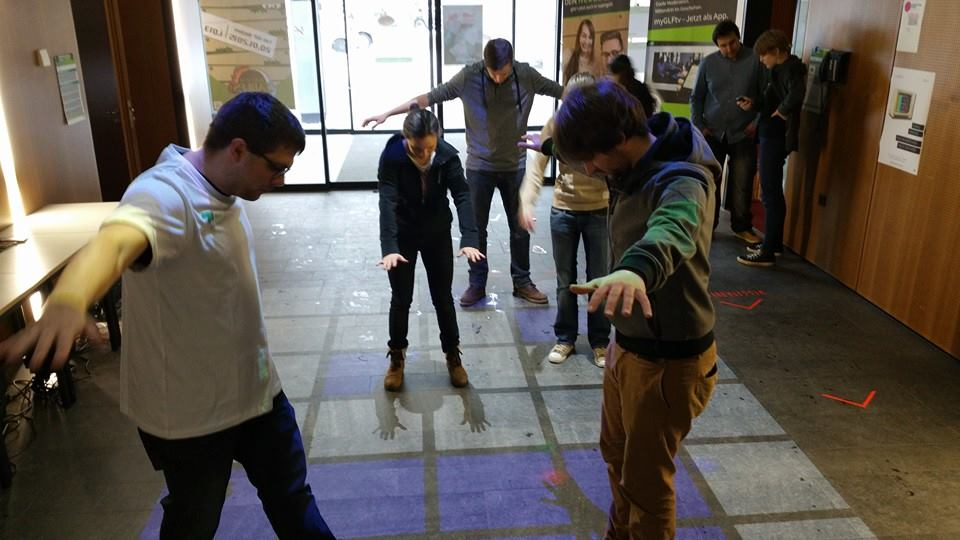
\includegraphics[width=0.9\textwidth]{images/TdM2.jpg}
	\caption{Erdgeschoss \textit{(Foto: Ramazan Gündogdu)}}
	\label{fig:TdM2}
\end{figure}

\begin{figure}[htbp]
	\centering
		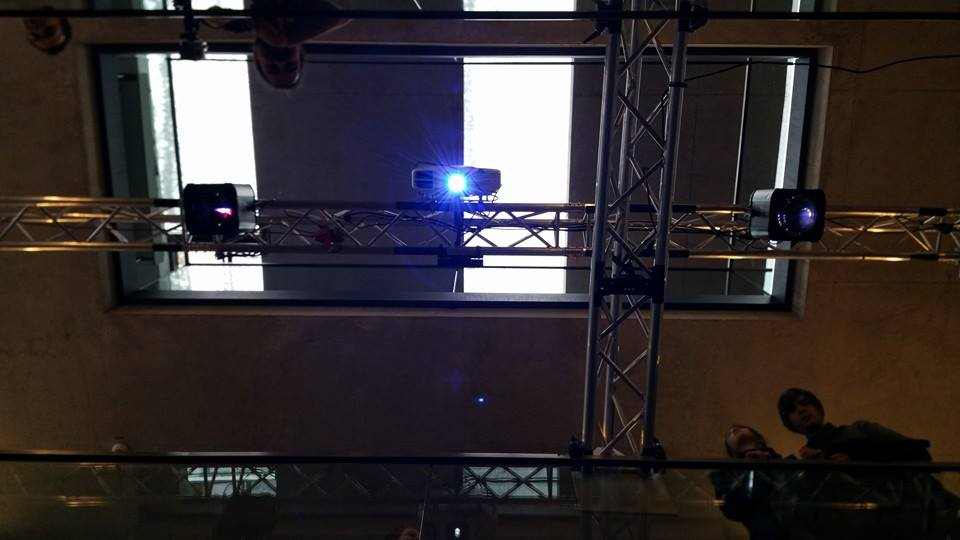
\includegraphics[width=0.9\textwidth]{images/TdM3.jpg}
	\caption{Traversenkonstruktion \textit{(Foto: Ramazan Gündogdu)}}
	\label{fig:TdM3}
\end{figure}

\begin{figure}[htbp]
	\centering
		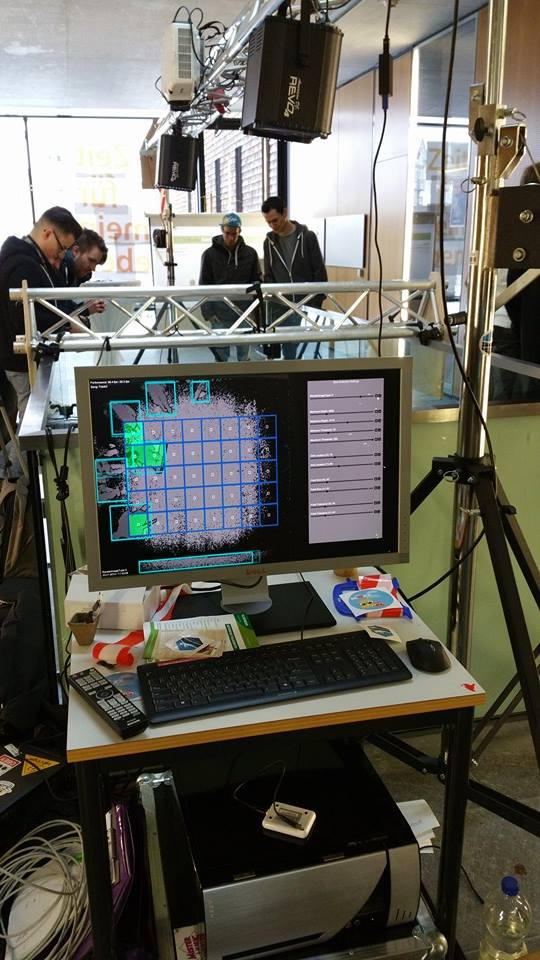
\includegraphics[width=0.9\textwidth]{images/TdM4.jpg}
	\caption{Erster Stock Kontrollprogramm \textit{(Foto: Ramazan Gündogdu)}}
	\label{fig:TdM4}
\end{figure}

\begin{figure}[htbp]
	\centering
		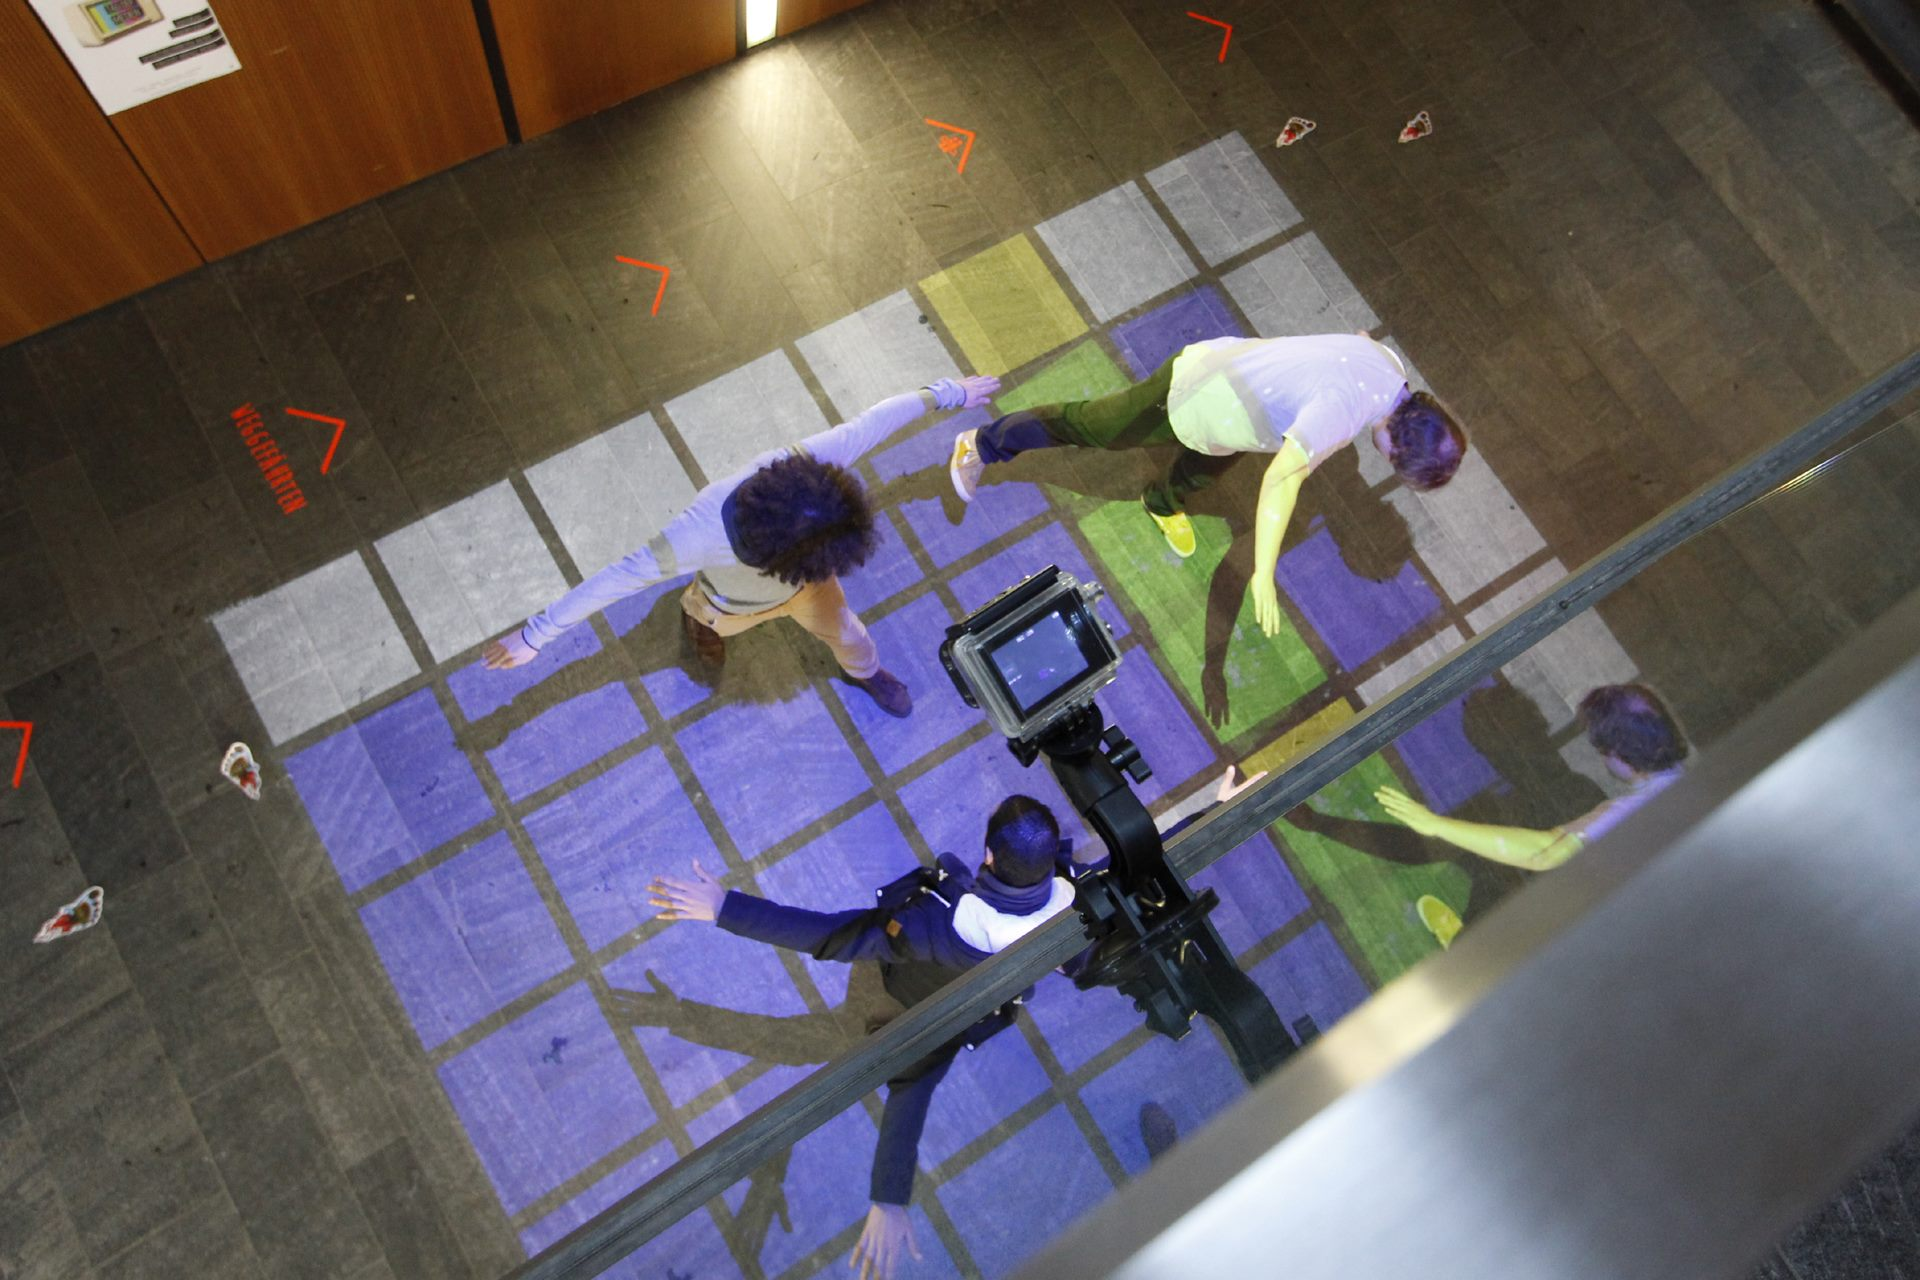
\includegraphics[width=0.9\textwidth]{images/TdM5.jpg}
	\caption{Installation im Einsatz \textit{(Foto: GLF TV)}}
	\label{fig:TdM5}
\end{figure}
\clearpage

\subsubsection{Impressionen Erste Tests}
Die Installation wurde schon Wochen vor dem Tag der Medien in verschiedenen Varianten aufgebaut und auch an anderen Orten, wie in der Aula, getestet.

\begin{figure}[htbp]
	\centering
		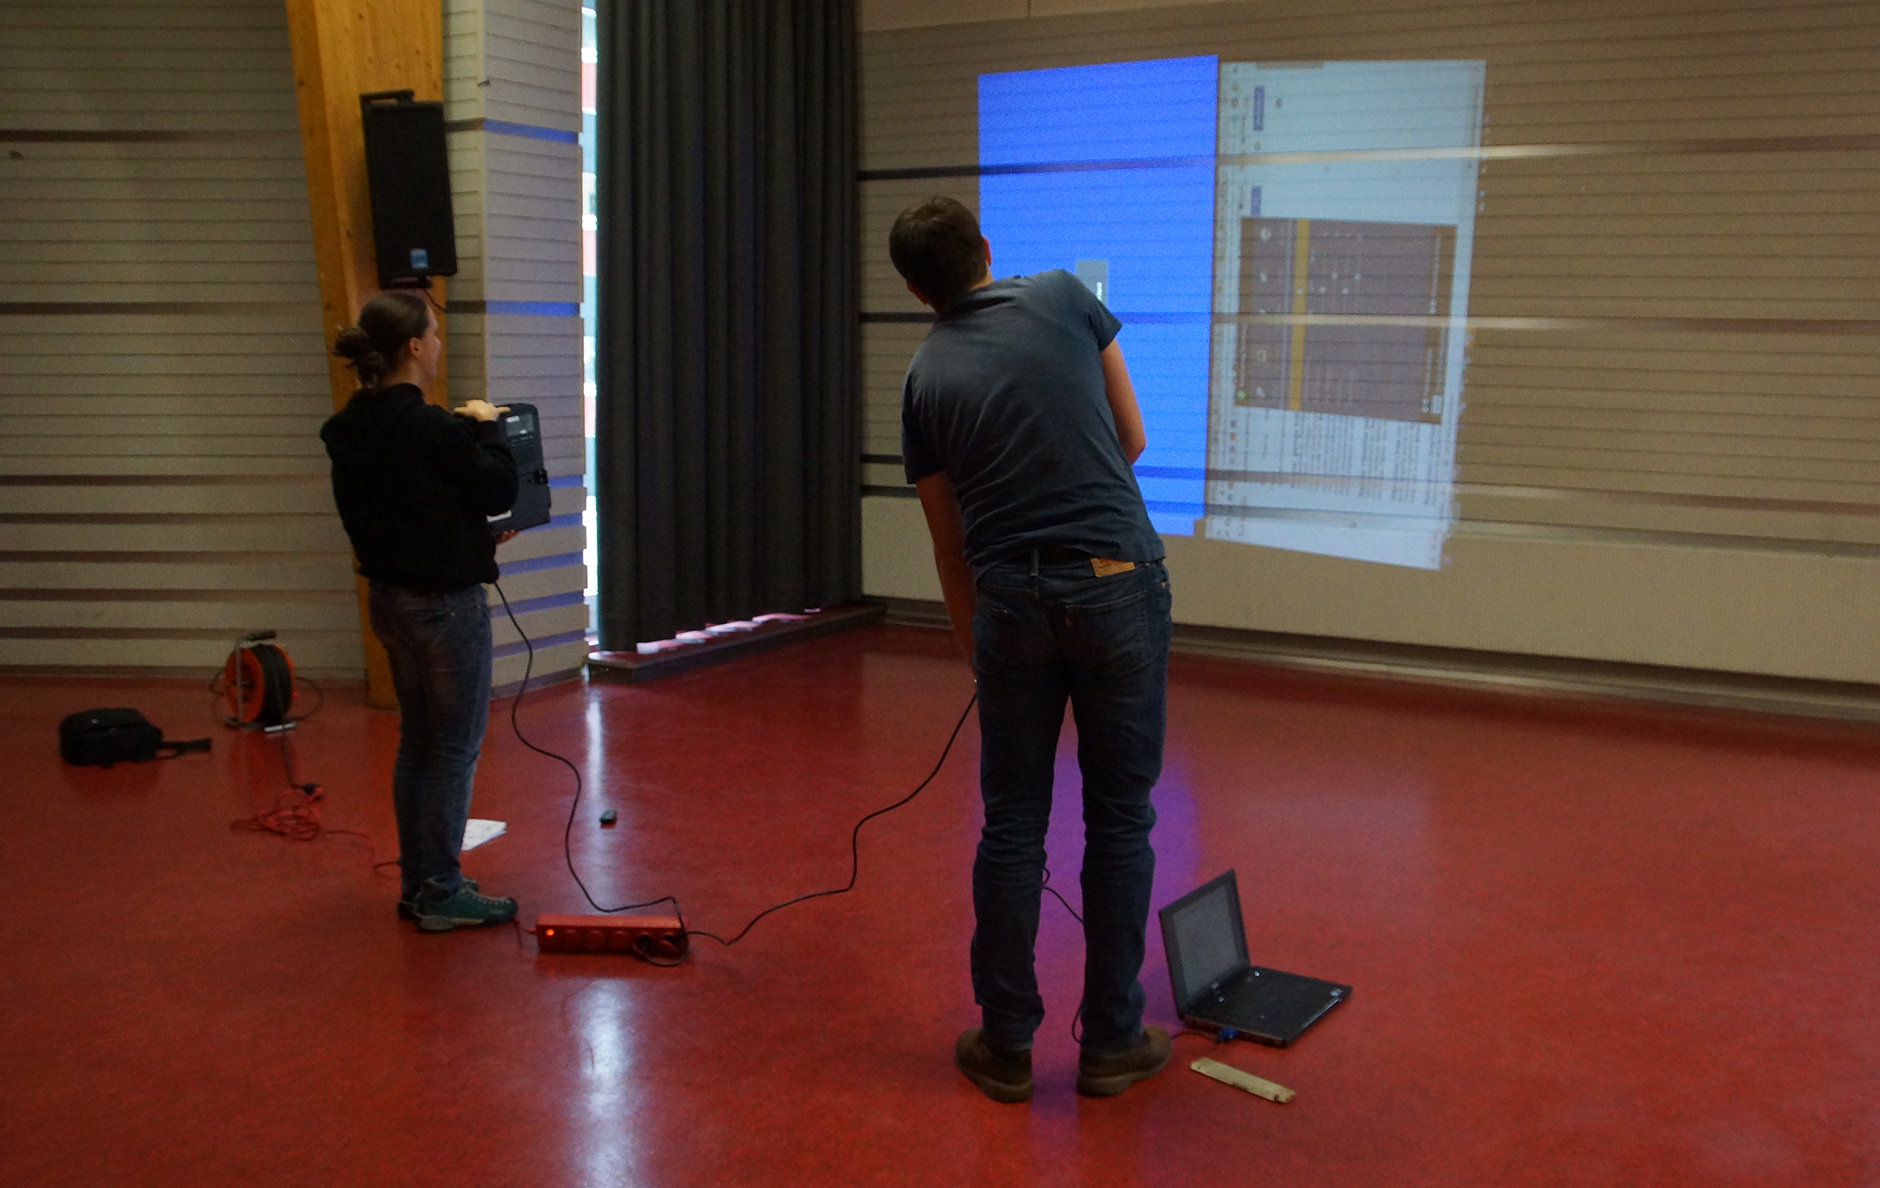
\includegraphics[width=0.9\textwidth]{images/Test1.png}
	\caption{Tests mit zwei Beamern in der Aula}
	\label{fig:Test1}
\end{figure}

\begin{figure}[htbp]
	\centering
		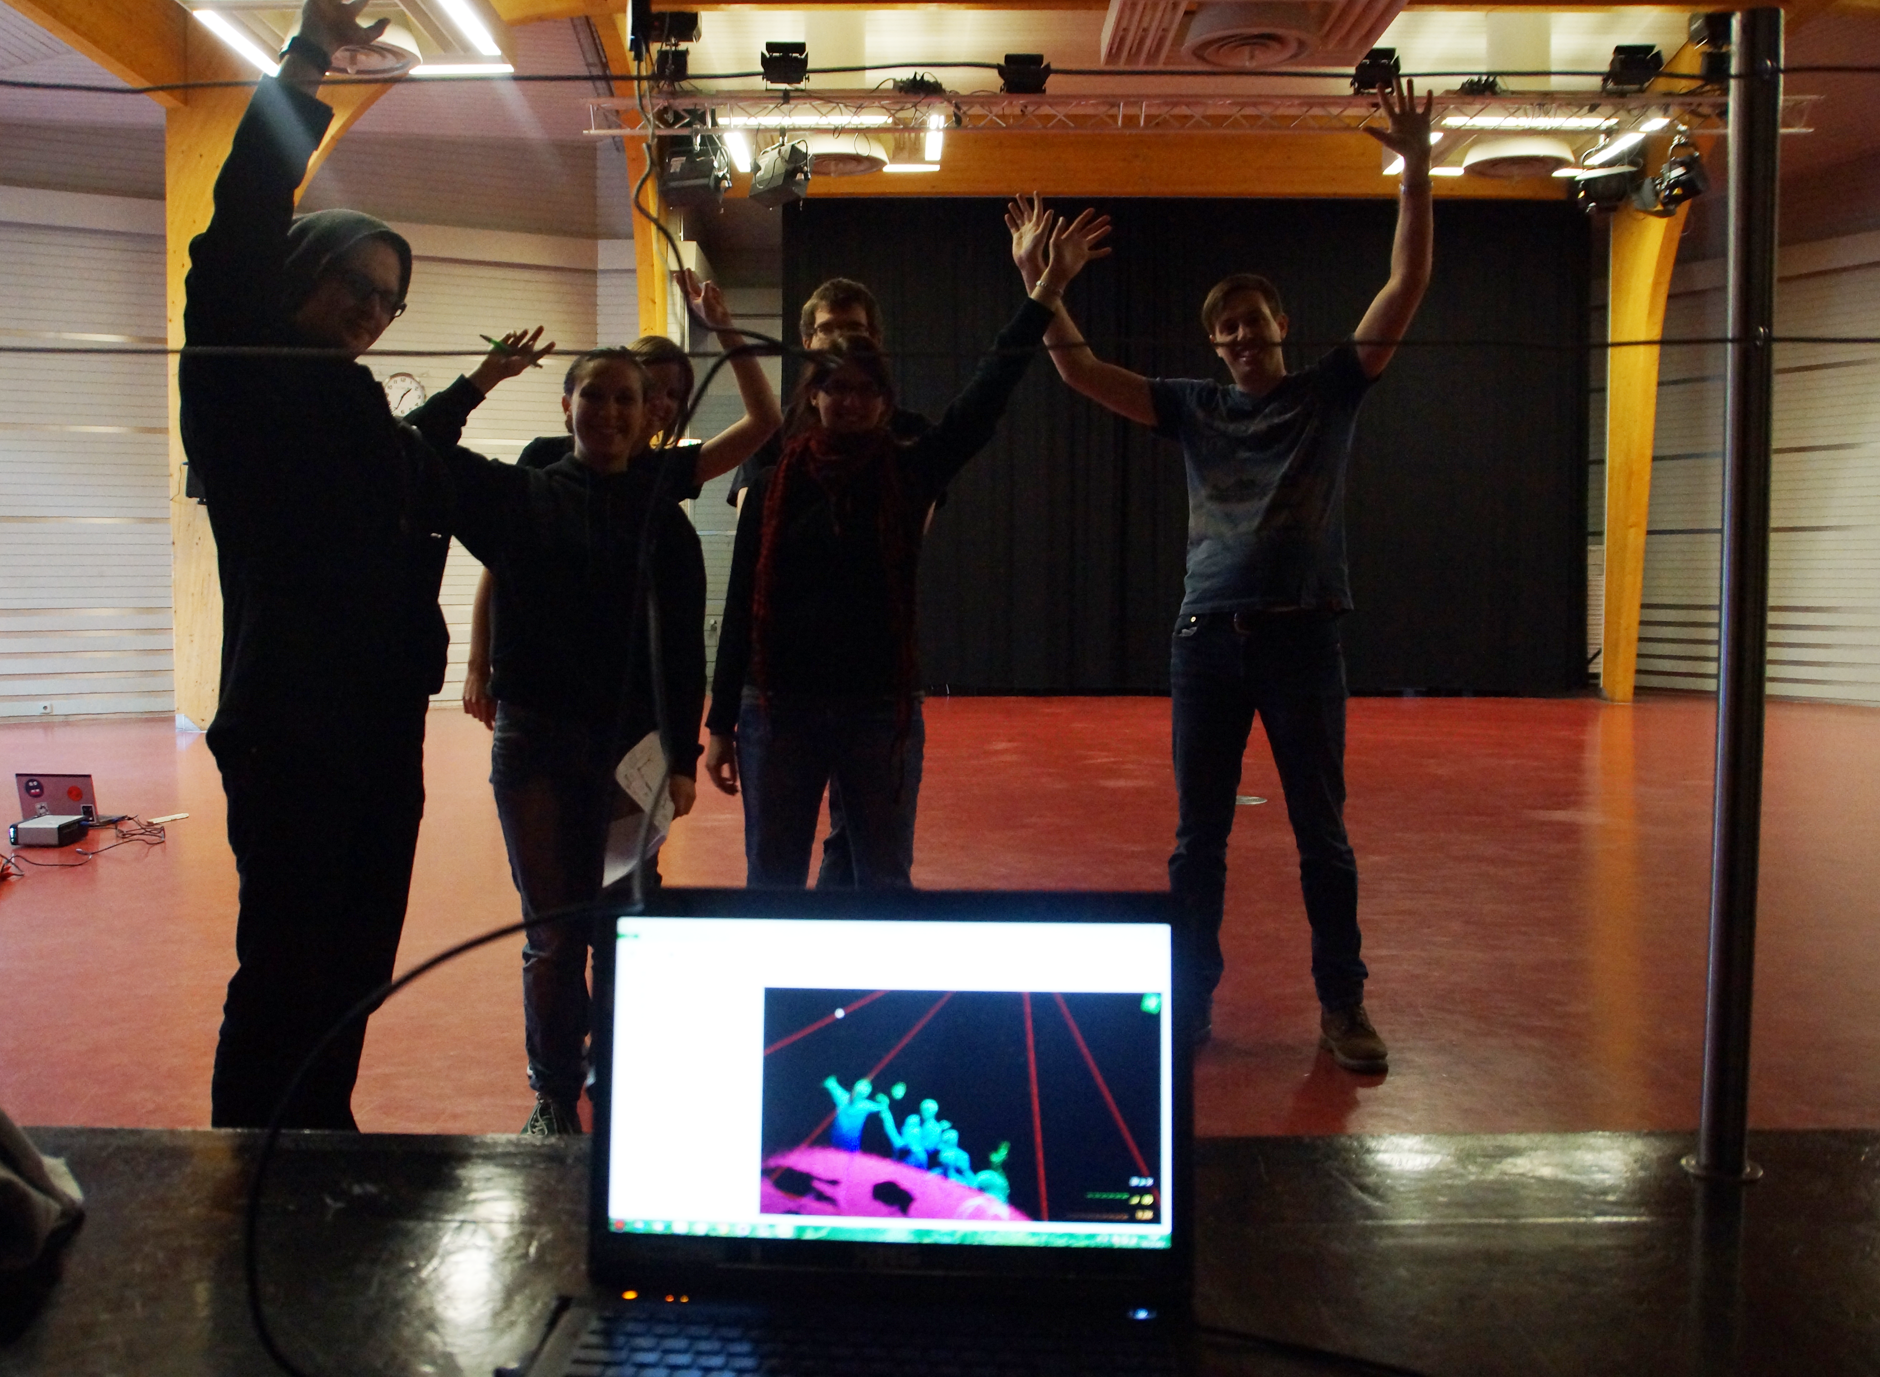
\includegraphics[width=0.9\textwidth]{images/Test2.png}
	\caption{Tests mit der Kinect in der Aula}
	\label{fig:Test2}
\end{figure}

\begin{figure}[htbp]
	\centering
		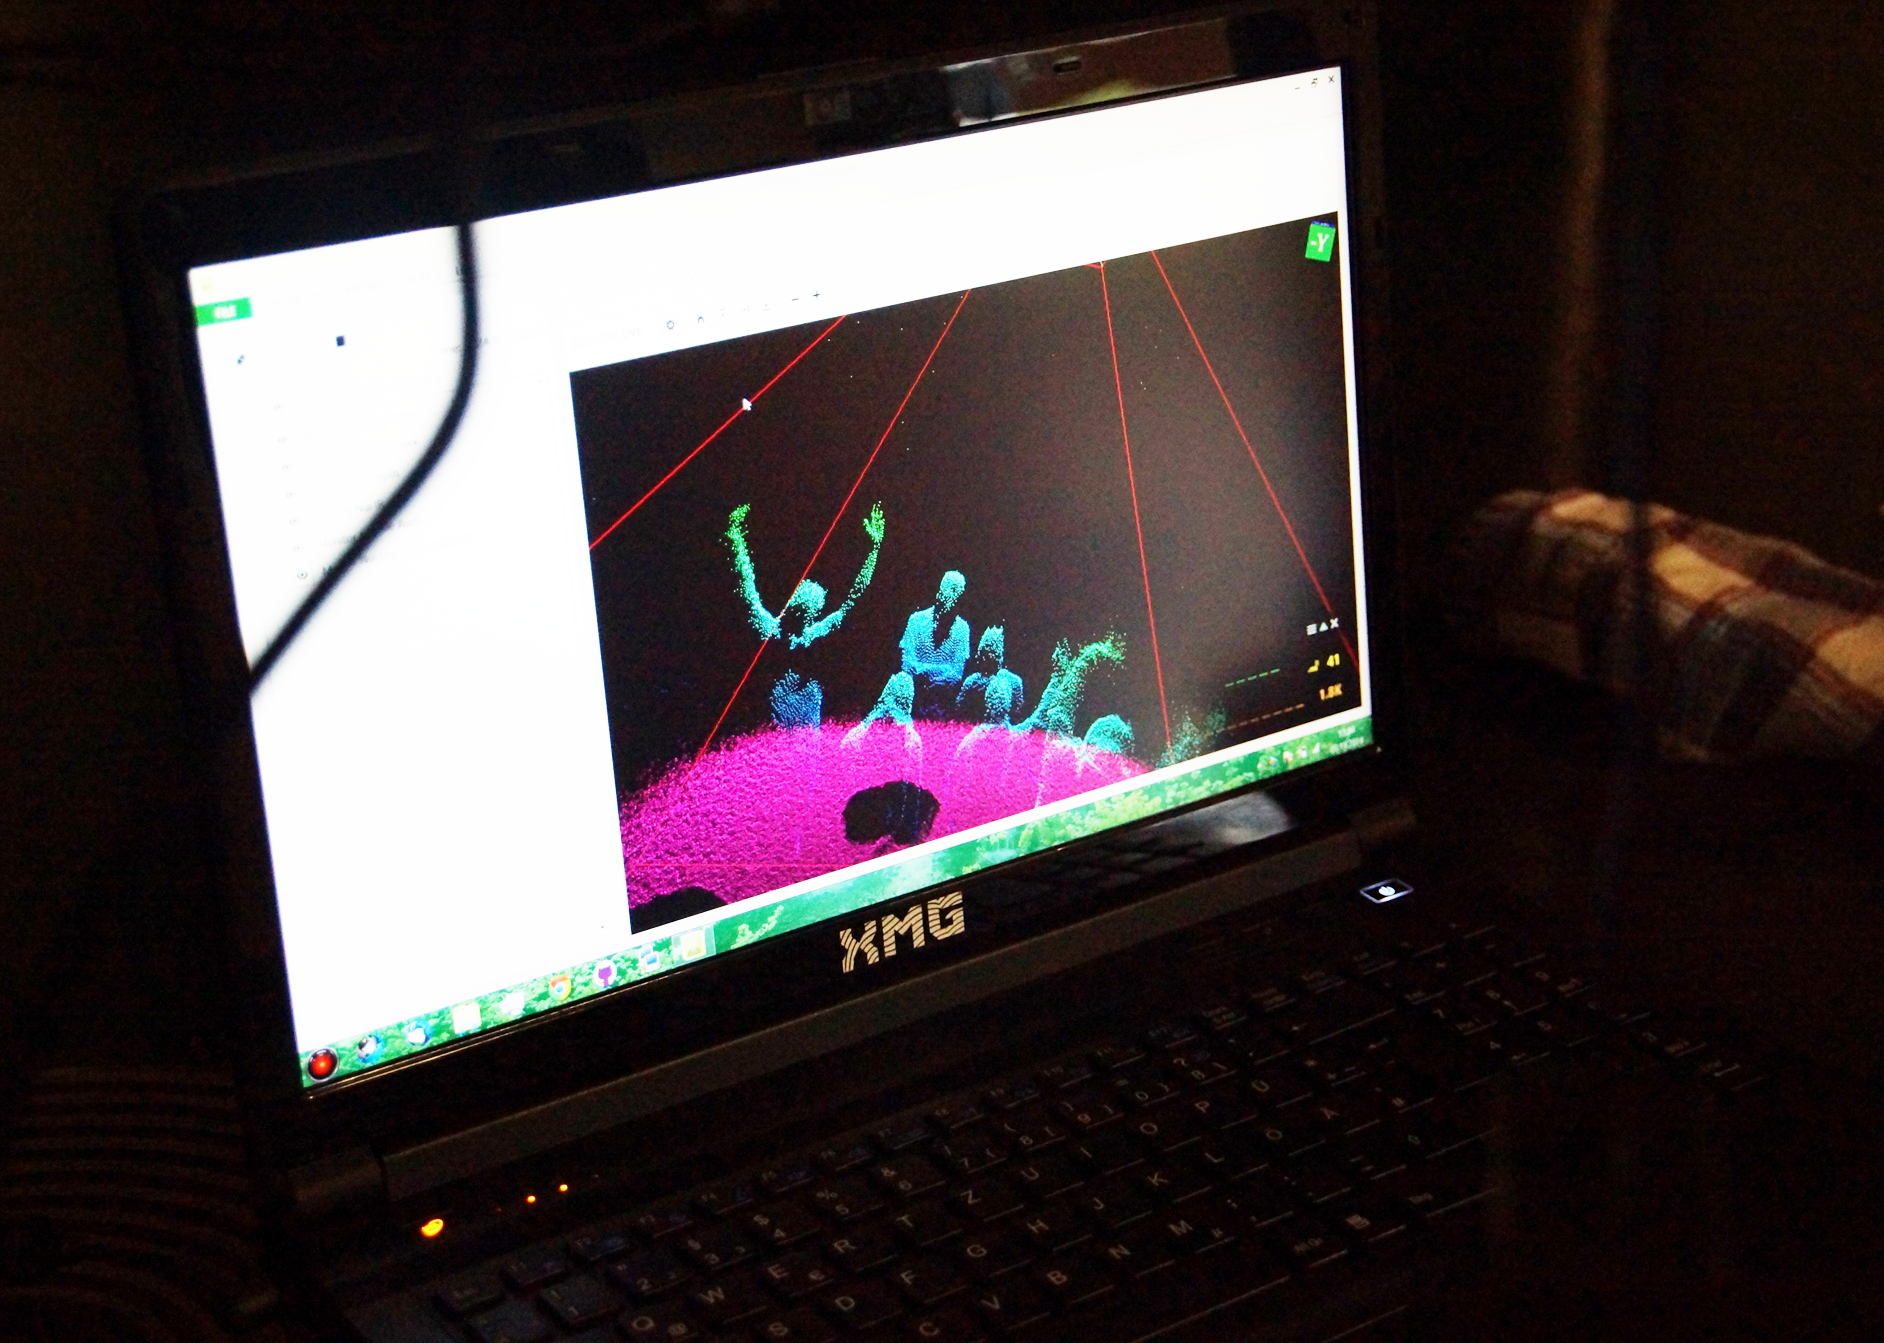
\includegraphics[width=0.9\textwidth]{images/Test3.png}
	\caption{Tests mit der Kinect in der Aula}
	\label{fig:Test3}
\end{figure}

\begin{figure}[htbp]
	\centering
		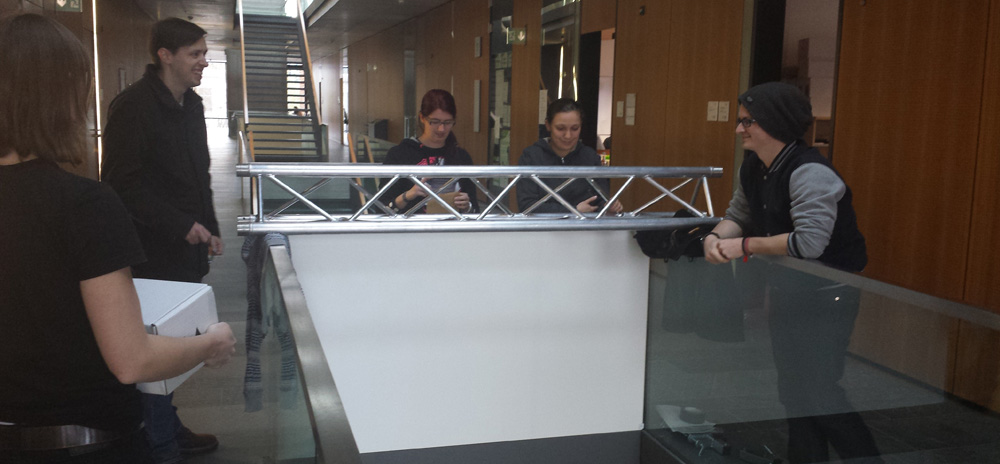
\includegraphics[width=0.9\textwidth]{images/Test4.jpg}
	\caption{Ertste Traversentests im I-Bau}
	\label{fig:Test4}
\end{figure}
\clearpage

\subsubsection{Technische Zeichnungen}

\end{document}